\chapter{Data Analysis}
\label{chap:ana}

%simultaneous in KK-mass bins and tagging categories

To extract the theoretical parameters that describe the \BstoJpsiKK{} decay from the experimental data, the model of decay time and decay
angles, as discussed in Chapter~\ref{chap:pheno}, is fitted to the distribution of decays in the data. Several experimental effects have to
be taken into account in this fit. Some of these effects, for instance the uncertainty in the measurement of the decay time, are included
by modifying the theoretical model. Backgrounds, on the other hand, are dealt with by selecting signal-like decay candidates in the data
and by subtracting remaining background from the data after selection.

This chapter deals with the preparation of experimental data (Section~\ref{sec:ana_bkgSub}) and the model that can be used to fit these
data (Sections~\ref{sec:ana_time}--\ref{sec:ana_tagging}). Also the use of the decay model in the fit (Section~\ref{sec:ana_fit}) and in
simulation (Section~\ref{sec:ana_sim}) are discussed.

\section{Maximum-Likelihood Fit}
\label{sec:ana_fit}

The fit of the decay model to the data is an \emph{unbinned maximum-likelihood fit}. A probability density function (PDF) is constructed by
normalizing the expression for the differential decay rate, including experimental effects, by dividing by its integral over decay time and
decay angles. A likelihood function of the PDF parameters for one $\Bs$ decay is given by the PDF at the values of time and angles for
that decay. The likelihood function for the full sample of decays is given by the product of all individual likelihoods.

Parameter values are estimated by maximizing the likelihood function for the sample. In practice, the negative logarithm of the likelihood
function (NLL) is minimized to find the maximum likelihood. Instead of a product, the NLL is a sum of the contributions from individual
decays.

The shape of the NLL around the minimum can be approximated by a second order Taylor series, i.e. a parabola. Since the first derivative of
this function vanishes at the point where the NLL reaches its minimum, the approximation for a given parameter $\mu$ can be written in the
form
\begin{equation}
  \label{eq:NLLPara}
  \text{NLL}(\mu) \approx \frac{1}{2\,\sigma_\mu^2}\, (\mu-\hat{\mu})^2 + C \ ,
\end{equation}
where $\hat{\mu}$ is the value of parameter $\mu$ in the minimum, $\sigma_\mu$ determines the width of the NLL shape around the minimum,
and $C$ is the NLL value in the minimum. The width, $\sigma_\mu$, is (related to) the statistical uncertainty of the estimate of parameter
$\mu$. The wider the NLL shape around the minimum, the larger the value of $\sigma_\mu$ and thus the uncertainty.

It depends on the actual shape of the NLL how well it is approximated by a parabola away from the minimum. An important factor is the
number of decays that is used to build the NLL. With more data the statistical uncertainties of the parameter estimates become smaller and,
in general, the NLL becomes more parabolic within an interval of a few times the value of $\sigma_\mu$ around the minimum.

In case the distribution of parameter estimates $\hat{\mu}$ from different measurements is described by a Gaussian shape, the shape of the
NLL will be truly parabolic. In this case the parameter $\sigma_\mu$ is an estimate of the standard deviation of the $\hat{\mu}$
distribution, which can be used as a measure of the statistical uncertainty of a parameter estimate. The value of $\sigma_\mu$ is
determined from the second derivative of the NLL, which is given by $\frac{1}{\sigma_\mu^2}$.

If the shape of the NLL around its minimum is not sufficiently parabolic, a different measure of the statistical uncertainty may be used.
Commonly the (absolute) difference between the value of $\mu$ at the point where the NLL reaches a value of $\tfrac{1}{2}+C$ and
$\hat{\mu}$ is taken as the uncertainty. In the parabolic case the NLL reaches this point at $\hat{\mu}+\sigma_\mu$ and
$\hat{\mu}-\sigma_\mu$, which results in an uncertainty of $\sigma_\mu$, as expected. In a more general case this NLL value may be reached
on the left and the right of $\hat{\mu}$ at different distances, which results in an asymmetric uncertainty.

In some cases the shape of the NLL differs from a parabola too much to give a meaningful single estimate of the parameter value and a
corresponding uncertainty. The simplest way to provide an estimate of the value in these cases is to specify the interval bounded by the
values of $\mu$ at a given NLL value. Common NLL values are the values that a parabola would reach at $n\cdot\sigma_\mu$ from the minimum,
which are given by $\tfrac{1}{2}\,n^2+C$. Hence the intervals are referred to as ``$n$ sigma'' intervals.

In general the NLL is a function of more than one parameter. The distribution of parameter estimates in the parabolic approximation is
given by a multivariate Gaussian shape, which includes also correlations between the estimates. Both the uncertainties and the correlations
of the parameter estimates are estimated from the shape of the NLL in the minimum, by determining second derivatives for all pairs
of parameters.

The parabolic shape of Equation~\ref{eq:NLLPara} for a parameter $\mu$ is given by the minimum of the NLL at each $\mu$ value. In the
parabolic approximation the minimum for a given value of $\mu$ is reached at
\begin{equation}
  \frac{1}{\sigma_{\nu_i}}\, (\nu_i-\hat{\nu}_i)  = \rho_{\mu\nu_i}\, \frac{1}{\sigma_\mu}\, (\mu-\hat{\mu})
\end{equation}
for all the other parameters $\nu_i$, where $\rho_{\mu\nu_i}$ is the correlation coefficient between the parameters $\mu$ and $\nu_i$. The
resulting function of parameter $\mu$ is termed \emph{profiled NLL}, the second derivative of which is again equal to
$\frac{1}{\sigma_\mu^2}$.


%%%%%%%%%%%%%%%%%%%%%%%%%%%%%%%%%%%%%%%%%%%%%%%
\subsection{Fit with Weighted Decay Candidates}
\label{subsec:ana_fit_weights}
%%%%%%%%%%%%%%%%%%%%%%%%%%%%%%%%%%%%%%%%%%%%%%%

As will be described in Section~\ref{sec:ana_bkgSub}, the time and angular distribution for \BstoJpsiKK{} signal decays is obtained by
subtracting the background distribution from the distribution that is observed in the data. This is accomplished by adding background
decay-candidates to the sample with negative weights. In the NLL, the contribution of each decay candidate is then multiplied with the
value of its weight.

Although the position of the minimum of a weighted NLL still gives a good estimate of the values of the NLL parameters, the parameter
uncertainties cannot be estimated directly from the shape of the NLL at its minimum any more. This can be seen by considering a fit in
intervals of a given variable, where the observed number of decays in each interval is compared to the prediction of this number by a
model. The uncertainties in the estimates of the model parameters are now related to the uncertainties in the observed number of decays in
each interval.

For unweighted decays the distribution of the observed number of decays ($N$) is a Poisson distribution, for which both the mean and the
variance are given by the expected number in the interval ($\nu$). An estimate of the expected number of decays, $\hat{\nu}$, is given by
$N$ and an estimate of the corresponding uncertainty by the square root of the estimated variance, $\sqrt{N}$.

In a fit with weighted decay candidates, where each candidate counts with a weight $w_c$, the observed number of decays is replaced by the
sum of weights, $W$\textequiv$\sum_c w_c$. The estimate of $\nu$ is now also given by $W$, as expected, but the uncertainty is estimated by
$\sqrt{W}$, which cannot be correct. If all weights are multiplied by a constant number, $n$, the relative uncertainty in the estimate of
$\nu$ should not change, since no information was added to the data sample. This means that the absolute uncertainty should increase by a
factor $n$, as $\hat{\nu}$\texteq$W$ does. If the uncertainty is estimated by $\sqrt{W}$, it only increases by a factor $\sqrt{n}$.

The correct uncertainty estimate for the expected number of decays is given by the square root of $W'$\textequiv$\sum_c w_c^2$. Unlike
$\sqrt{W}$, $\sqrt{W'}$ increases by a factor $n$ if all weights are multiplied by this common factor. To obtain this estimate of the
uncertainty, the original estimate from the Poisson distribution should be divided by a factor $\sqrt{\alpha}$, where $\alpha$ is given by
\begin{equation}
  \alpha \equiv \frac{W}{W'} = \frac{\sum_c w_c}{\sum_c w_c^2} \ .
\end{equation}

In an unbinned maximum likelihood fit the correction factor $\alpha$ can be used to modify the shape of the NLL. Since the uncertainties
are estimated from the second derivatives of the NLL, which are given by $\frac{1}{\sigma_\mu^2}$ in the parabolic case, the NLL is
multiplied by a factor $\alpha$:
\begin{equation}
  \label{eq:NLLPara_alpha}
  \text{NLL}'(\mu) \approx \frac{\alpha}{2\,\sigma_\mu^2}\, (\mu-\hat{\mu})^2 + C' \ .
\end{equation}
This will make the shape of the parabola around the NLL minimum wider (if $\alpha$\textlt1) or narrower (if $\alpha$\textgt1). Notice that
this does not affect the position of the minimum, from which the parameter values are estimated.

Note that whereas the factor $\alpha$ is an exact correction for the uncertainty estimate of the expected number of decays in the above
example, it is only an approximate correction for the parameters in the NLL. The resulting uncertainties have to be checked by evaluating
the shape of the distribution of parameter estimates in simulated experiments, as will be discussed in Sections~\ref{sec:ana_sim} and
\ref{sec:result_paramEst}.

\section{Decay-Candidate Selection and Background}
\label{sec:ana_bkgSub}
%show mass-fit results in $\cthetal$ bins

While the decay model discussed in Chapter~\ref{chap:pheno} describes the \BstoJpsiKK{} signal, the time and angular distribution in the
experimental data contains both signal and background decay candidates. The background distribution is subtracted from the total
distribution in the data to be able to fit the model to the signal distribution. Since there are statistical uncertainties associated to
both the total distribution and the subtracted background distribution, however, the resulting uncertainties in the signal-parameter
estimates become larger with an increasing amount of background decay candidates. Therefore, a selection procedure is applied, designed to
reject as many background candidates as possible without removing too many signal candidates.


%%%%%%%%%%%%%%%%%%%%%%%%%%%%%
\subsection{Selection}
\label{subsec:ana_bkgSub_sel}
%%%%%%%%%%%%%%%%%%%%%%%%%%%%%

The decay-candidate selection procedure is briefly described here. See reference~\cite{Aaij:2015} for a detailed discussion.

As described in Section~\ref{subsec:intro_LHCb_Jpsiphi}, the first selection requirements are applied in the L0 trigger, which only selects
events with hits in the LHCb muon stations and particles with a sufficiently high (transverse) momentum. From the events that remain, the
HLT reconstructs and selects $\mumu$ pairs that are likely to originate from a $\Jpsi\to\mumu$ decay. Offline, the resulting
$\Jpsi\to\mumu$ candidates are matched to $\KK$ pairs to form \BstoJpsiKK{} decay candidates. The four tracks these candidates consist of
are required to be compatible with a $\Bs$ that was produced in the associated primary vertex and decayed at a decay time above a given
threshold.

In both HLT1 and HLT2 there are two different types of selections applied. The first type does not use any information on the distance that
the $\Bs$ travelled before it decayed and the second type does. Requiring a minimum flight distance reduces the fraction of
background candidates significantly, since all four tracks originate from the primary vertex for most combinatorial background, while the
tracks in a $\Bs$ decay originate from a secondary vertex at some distance from the primary vertex. However, the flight distance variable
is correlated with the decay time variable and requiring a minimum flight distance introduces a non-trivial selection efficiency as a
function of decay time. Therefore, the sets of selection criteria that use information on the flight distance are called \emph{decay-time
biasing} or \emph{biased}.

The unbiased HLT1 selection requires two oppositely charged muon candidates that are close enough to originate from one decay vertex and
have a $\mumu$ invariant mass greater than 2.7\unitsp\GeV. The biased HLT1 selection does not require a $\Jpsi$ candidate, but selects
single tracks with a perpendicular distance to any primary vertex greater than 0.1\unitsp{}mm. Both of these selections reduce the number
of selected events to a manageable level. Approximately 68\% of the decay candidates that are finally used in the fit is selected by both
the unbiased and biased selections, approximately 14\% exclusively by the unbiased selection, and approximately 19\% exclusively by the
biased selection.
% HLT1: 81% unbiased; about the same numbers for the signal

Both the unbiased and the biased HLT2 selections require $\Jpsi\to\mumu$ candidates with an invariant $\mumu$-mass within a window of
0.24\unitsp\GeV{} centred at the $\Jpsi$ mass of 3.10\unitsp\GeV. In addition, the biased selection requires a minimum \emph{decay-length
significance} (DLS) of three for the $\Jpsi$ candidate. The DLS is defined as the distance between the $\mumu$ vertex and the associated
primary vertex (\emph{decay length}) divided by the uncertainty on this distance. Since the decay length is a measure of the flight
distance of the $\Bs$, this requirement is decay-time biasing.

Without the minimum-DLS requirement the rate of events that pass the HLT2 selection would be too high to handle online. Therefore, the
rate of the unbiased selection is reduced by processing only a fraction of the events that pass the HLT1 selection. To keep the selection
unbiased, the processed events are randomly selected, without considering any information on the reconstructed particles. In the final
data sample that is used in the fit, the number of decay candidates that is exclusively selected by the unbiased HLT2 selection is three
per cent of the number of candidates selected by the biased selection. Considering only signal candidates, the unbiased HLT2 selection adds
one per cent to the total.

The method of modelling the non-trivial decay-time efficiency shape introduced by the biased HLT selections is discussed in
Section~\ref{subsec:ana_time_acc}. Because the unbiased HLT2 selection adds only few signal candidates to the final data sample, but
including these data complicates modelling of the efficiency significantly, only the time and angular distributions of HLT2-biased
candidates are fitted. However, candidates selected by the unbiased HLT2 selection are used to extract the efficiency shapes from the
\BstoJpsiKK{} data. The efficiencies of the biased selections are determined relative to the uniform efficiencies of the unbiased
selections. 

In the offline reconstruction process the muon tracks and the $\mumu$ vertex of $\Jpsi\to\mumu$ candidates selected by HLT2 are combined
into \BstoJpsiKK{} candidates with two oppositely charged kaons that form a $\KK$ vertex. The subsequent stripping selection imposes
requirements on how well detector hits form tracks within experimental uncertainties, how well tracks form $\mumu$, $\KK$, and $\mumu\,\KK$
vertices, the particle transverse momenta, the likelihood that the particles are identified correctly as muons and kaons, the invariant
masses of the reconstructed $\mumu$, $\KK$, and $\JpsiKK$ combinations, and the decay time of the candidate. About twelve million
\BstoJpsiKK{} candidates remain after this selection stage.

The selection of decay candidates is refined in the final offline stage. To visualize the effect of the selection, the distribution in
$\JpsiKK$ mass of remaining decay candidates is plotted for different selection requirements in Figure~\ref{fig:JpsiKKMassSel}. Notice that
the figure shows only a part of the mass range.
\begin{figure}[tb]
  \centering
  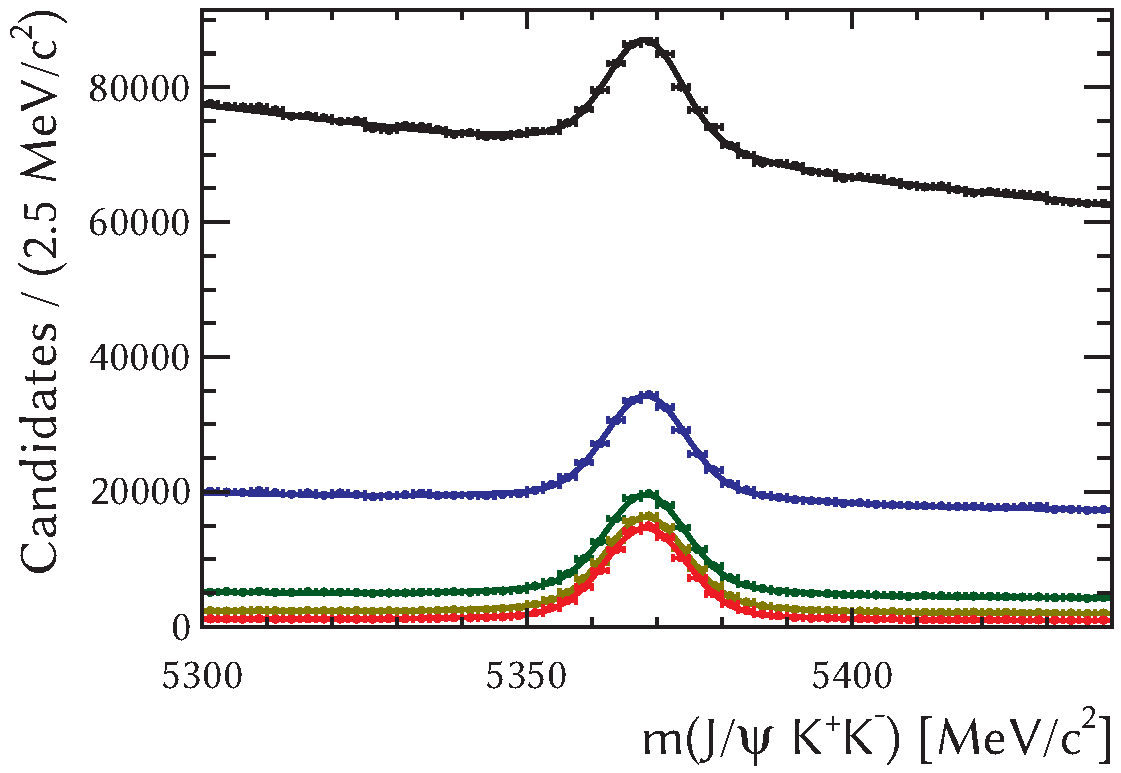
\includegraphics[width=0.7\textwidth]{graphics/analysis/JpsiKKMassSel}
  \caption{Distribution of \BstoJpsiKK{} decays in $\JpsiKK$ mass for different selection criteria.
           The data are shown as points, while the lines represent a model that consists of the sum of two Gaussian shapes (signal)
           and an exponential shape (combinatorial background).
           Subsequent selection criteria are applied in addition to previous criteria:
           black: stripping selection; blue: minimum quality of $\Bs$ decay-vertex reconstruction;
           green: minimum $\KK$ transverse momentum; yellow: minimum decay time; red: full offline selection.
           Notice that only a part of the total mass range is shown.}
  \label{fig:JpsiKKMassSel}
\end{figure}

For \BstoJpsiKK{} signal candidates this distribution is a peak around the value of the $\Bs$ mass of approximately 5367\unitsp\MeV. The
width of this peak is determined by the experimental resolution on the $\JpsiKK$-mass measurement. The background is mainly combinatorial
and follows an exponential distribution, which decays slowly across the considered mass range. Because of the obvious difference in
distributions of $\JpsiKK$ mass for the signal and the background, this variable can be used to statistically separate the two
contributions.

The distribution of black data points in Figure~\ref{fig:JpsiKKMassSel} is for candidates that pass the stripping selection without further
requirements. A peak of signal candidates is visible on top of a large background distribution. To determine the numbers of signal and
background candidates, the surface areas underneath the peak and the exponential distribution are determined with a fit. The signal peak is
modelled with the sum of a narrow ($\sigma$\textapprox6\unitsp\MeV) and wide ($\sigma$\textapprox16\unitsp\MeV) Gaussian shape and the
background with and exponential shape. The fit yields approximately 123 thousand signal candidates, which corresponds to a signal fraction
of approximately one per cent.

In the rest frame of the $\Bs$, the momentum of the $\KK$ pair is approximately 1.6\unitsp\GeVc{} for signal decays. Boosting into the
frame of the detector, approximately along the beam axis, this translates in a typical transverse momentum above 1\unitsp\GeVc. The sum of
the transverse momentum components of two kaons that accidentally form a suitable $\KK$ vertex in combinatorial background is often not
sufficient to make a transverse momentum of 1\unitsp\GeVc. As a result, requiring this value as a minimum in the offline selection removes
about 74\% of the background, but only 6\% of the signal, with respect to the stripping selection where already a minimum of
0.5\unitsp\GeVc{} was required. The $\JpsiKK$-mass distribution with the $\KK$ transverse momentum requirement is shown by the blue points
in Figure~\ref{fig:JpsiKKMassSel}.

To estimate the position of the $\Bs$ decay vertex and the kinematics of the particles in the decay as well as possible, these variables
are determined from a fit. The fit takes the position of the primary vertex, the muon and kaon tracks, and the corresponding experimental
uncertainties as inputs and minimizes a $\chi^2$ function for the position of the decay vertex and its perpendicular distance to the flight
path of the $\Bs$, which should be equal to zero. The value of the $\chi^2$ function in its minimum is a measure of the quality of the fit,
i.e. of how well the four reconstructed particles form a $\Bs$ decay vertex. The fit will in general be good for signal candidates, which
results in small values for the $\chi^2$ function.

Requiring a $\chi^2$ smaller than five times the number of degrees of freedom in the vertex fit removes about 75\% of the background that
remains after requiring a minimum $\KK$ transverse momentum of 1\unitsp\GeVc. Approximately 8\% of the remaining signal is lost. The
distribution of decay candidates after the $\KK$ transverse momentum and vertex fit quality requirements is shown by the green points in
Figure~\ref{fig:JpsiKKMassSel}.

A third requirement that removes a significant part of the background is a minimum on the reconstructed value of the decay time. For most
of the background candidates the four particles originate directly from the primary vertex, which corresponds to vanishing decay time
within experimental resolution. The stripping selection already requires a minimum decay time of 0.2\unitsp{}ps. Requiring a minimum of
0.3\unitsp{}ps in addition to the stripping selection and the $\KK$ transverse momentum and vertex fit $\chi^2$ requirements removes about
54\% of the remaining background and 6\% of the signal. The distribution for remaining candidates is shown by the yellow points in
Figure~\ref{fig:JpsiKKMassSel}.

Finally applying the full offline selection removes another 62\% of the background and 6\% of the signal, leaving approximately 94
thousand signal candidates and 135 thousand background candidates for further analysis. This corresponds to a signal fraction of 41\% in
the full $\JpsiKK$-mass range of 5200--5550\unitsp\MeV{} after the full selection.

The final $\JpsiKK$-mass distribution is shown by the red points in Figure~\ref{fig:JpsiKKMassSel} and also in
Figure~\ref{fig:JpsiKKMass_DG}. The latter figure shows the distribution both in the 5300--5440\unitsp\MeV{} mass range on a linear
vertical scale (left) and in the full mass range on a logarithmic vertical scale. The signal and combinatorial background contributions as
determined in the fit are shown separately.

\begin{figure}[tb]
  \centering
  \begin{subfigure}{0.49\textwidth}
    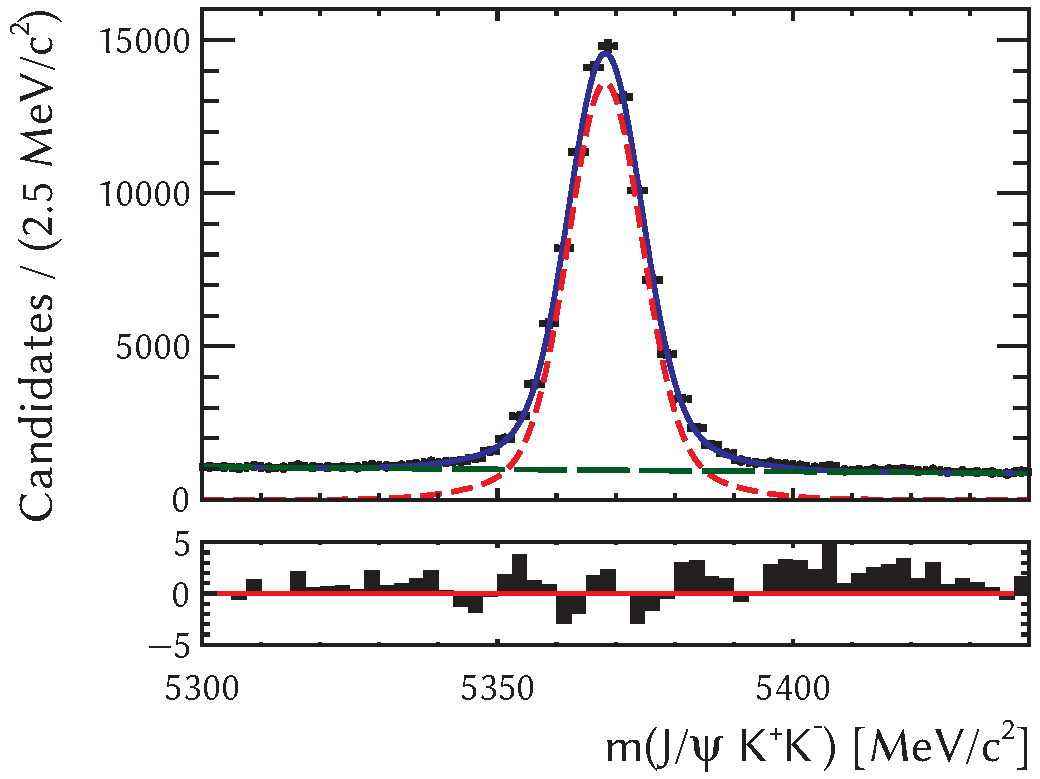
\includegraphics[width=\textwidth]{graphics/analysis/JpsiKKMass_DG_lin_resid}
    \caption{}
    \label{fig:JpsiKKMass_DG_lin}
  \end{subfigure}%
  \hfill%
  \begin{subfigure}{0.49\textwidth}
    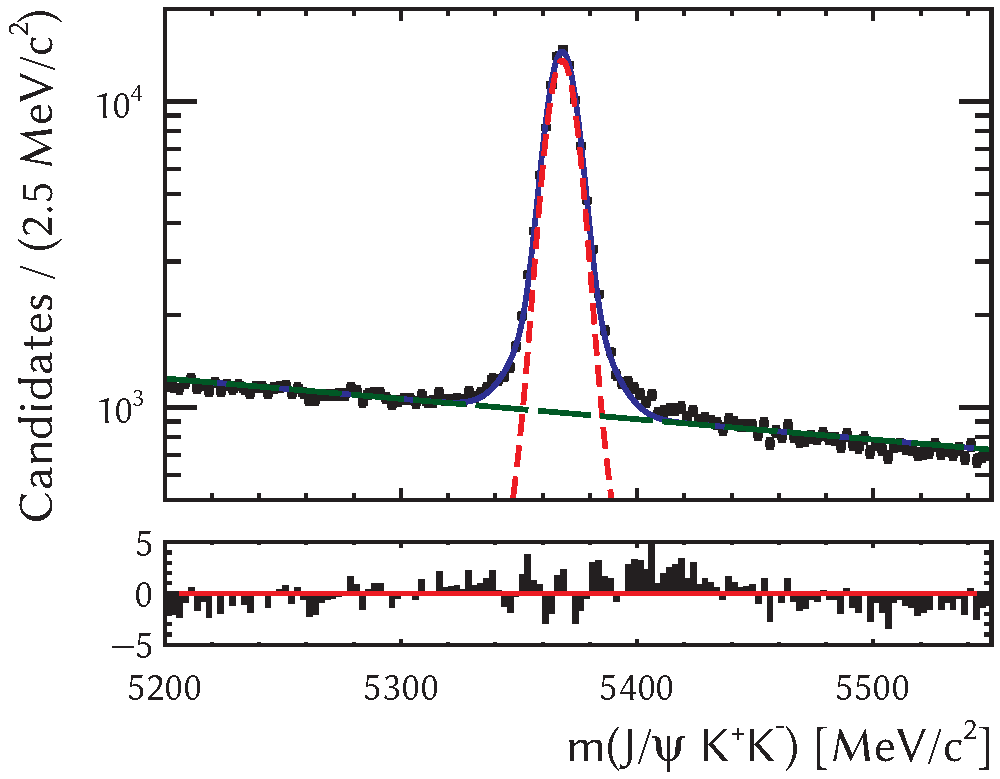
\includegraphics[width=\textwidth]{graphics/analysis/JpsiKKMass_DG_log_resid}
    \caption{}
    \label{fig:JpsiKKMass_DG_log}
  \end{subfigure}%
  \caption{Distribution of \BstoJpsiKK{} decay candidates in $\JpsiKK$ mass in
           (a) the signal mass range and
           (b) the full mass range on a logarithmic vertical scale.
           The black points show the distribution of the data and the blue, solid line shows a model that was fitted to the data.
           The model is the sum of two Gaussian shapes for the signal (shown by the red, short-dashed line)
           and an exponential shape for combinatorial background (shown by the green, long-dashed line).}
  \label{fig:JpsiKKMass_DG}
\end{figure}

In the areas below the $\JpsiKK$-mass distributions in Figure~\ref{fig:JpsiKKMass_DG} the corresponding \emph{residuals} are shown for each
mass bin. The residual is defined as the difference in values for the data and the (average) PDF in the bin, divided by the statistical
uncertainty of the data value. It is randomly distributed and quantifies how well the model describes the data in each bin. The residuals
in Figure~\ref{fig:JpsiKKMass_DG_log} seem to indicate a problem with the mass model, since the PDF generally underestimates the number of
decay candidates in the region of the signal peak, while it overestimates the number of candidates at the edges of the mass range. This
issue is mainly caused by misidentified backgrounds and will be addressed in Section~\ref{subsec:ana_bkgSub_bkgSub}.

Notice from Figures~\ref{fig:JpsiKKMassSel} and \ref{fig:JpsiKKMass_DG} that the signal candidates are concentrated in a mass window of
approximately 60\unitsp\MeV, centred at the $\Bs$ mass, where the signal fraction is approximately 80\%. The regions to the left and the
right of this \emph{signal window} are called mass \emph{side bands} and contain mainly background candidates. The candidates in the side
bands are used to estimate the time and angular distribution of the combinatorial background and subtract this from the total distribution
in the signal window to obtain the signal distribution. This procedure is described in the following section.


%%%%%%%%%%%%%%%%%%%%%%%%%%%%%%%%%%%
\subsection{Background Subtraction}
\label{subsec:ana_bkgSub_bkgSub}
%%%%%%%%%%%%%%%%%%%%%%%%%%%%%%%%%%%

The distribution of background decay candidates that remain after selection is subtracted from the total distribution by including
background candidates with negative weights in the data sample. For combinatorial background the most straightforward method of doing this
would be to give candidates in the signal region a weight equal to plus one and candidates in the $\JpsiKK$-mass side bands a small
negative weight, such that the contributions of background in the signal and side-band regions exactly cancel. Note that this assumes that
the background distribution in all variables of interest does not depend on the $\JpsiKK$ mass.

Because the definitions of the signal and side-band regions are rather arbitrary, a more sophisticated technique is applied. Although the
bulk of the signal decay candidates have a reconstructed $\JpsiKK$ mass in a region of approximately 60\unitsp\MeV{} around the $\Bs$ mass,
the tails of the signal mass distribution stretch beyond this mass window. Moreover, at the edges of the signal window the contribution of
background is larger than in the centre. To take these features of the mass distribution into account and estimate the contribution of
combinatorial background in the most optimal way, the candidate weights are not binary, but take a different value at each point in
$\JpsiKK$ mass.

The weights for subtracting combinatorial background are computed with the \splot/\sfit{} technique~\cite{Pivk:2004ty,*Xie:2009rka}, which
takes the $\JpsiKK$-mass distributions of the signal and the background as inputs. The resulting candidate weights are called
\emph{\sweight[s]}, which are larger than one in the centre of the signal peak and gradually become smaller away from the peak until they
are negative in the side bands.

The \splot/\sfit{} method assumes that, in addition to the background distribution, also the signal distribution in the variables of
interest does not depend on the $\JpsiKK$ mass. In other words, there can be no correlations between the $\JpsiKK$ mass and any other
variable that is to be analysed, for both the signal and the background distribution (but not their sum).

Before fitting the distribution of signal and combinatorial-background candidates and computing \sweight[s], the contributions from other
backgrounds are subtracted by adding decay candidates with negative weights to the data sample. Two additional backgrounds are considered,
both originating from the misidentification of particles in the detector: \BdtoJpsiKstKpi{} and \LbtoJpsipK. Because the detected particles
for these processes originate from decays of unstable particles (resonances), these contributions are also called \emph{resonant
backgrounds}.

\begin{figure}[tb]
  \centering
  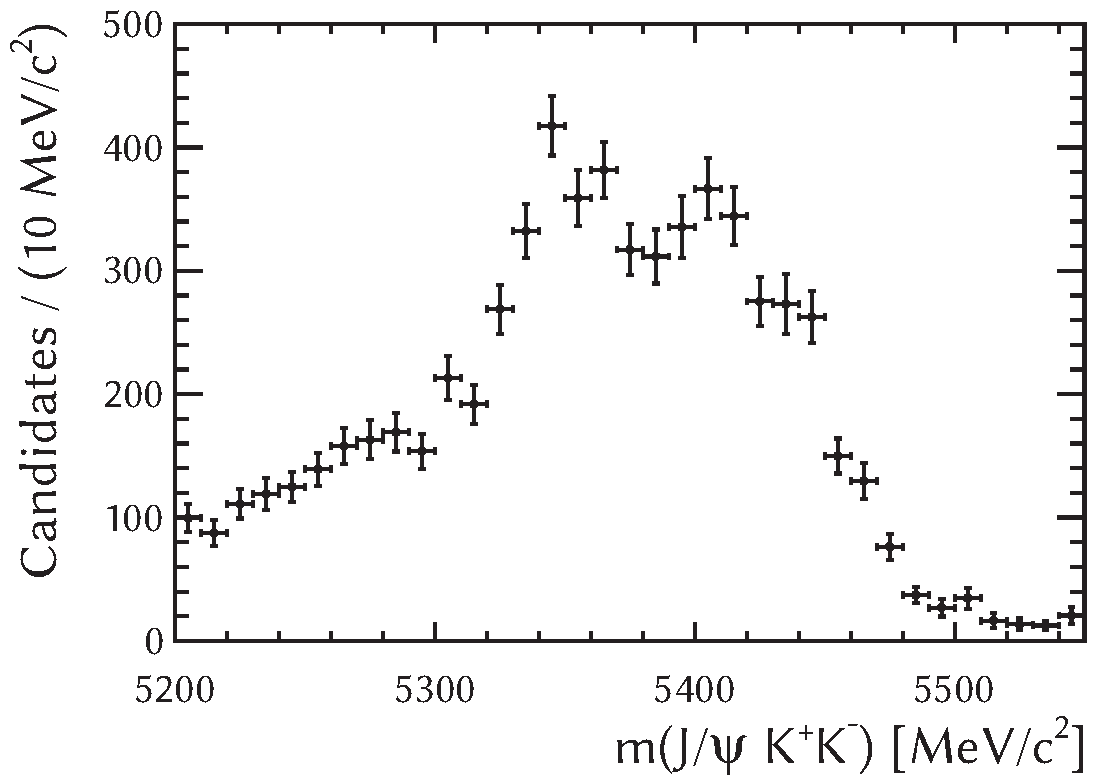
\includegraphics[width=0.5\textwidth]{graphics/analysis/JpsiKKMass_peakBkg}
  \caption{Distribution of weighted simulated resonant-background \BstoJpsiKK{} decay candidates in $\JpsiKK$ mass in the full mass range.}
  \label{fig:JpsiKKMass_peakBkg}
\end{figure}

Figure~\ref{fig:JpsiKKMass_peakBkg} shows the sum of the reconstructed $\JpsiKK$-mass distributions for the two resonant backgrounds. They
form a broad structure, without features that clearly distinguish these backgrounds from the signal and from combinatorial background.
Therefore, the resonant backgrounds are subtracted by adding simulated \BdtoJpsiKstKpi{} and \LbtoJpsipK{} decay candidates to the data
sample with negative weights that represent the amount of real resonant-background data, in total approximately seven thousand candidates.
Uncertainties in the numbers of background candidates and their distributions lead to systematic uncertainties in the final parameter
estimates, as will be discussed in Section~\ref{sec:result_syst}.

The $\JpsiKK$-mass distribution after subtracting the two resonant backgrounds is shown in Figure~\ref{fig:JpsiKKMass_DG_bkgSub}. Comparing
to Figure~\ref{fig:JpsiKKMass_DG}, it can be seen from the residuals that the PDF follows the data more closely. The systematic
underestimates of the numbers of decay candidates in the signal region and the overestimates in the side-band regions have reduced. It
appears, however, that this effect is still partially present. Moreover, the residuals in the signal region seem to be large than one would
expect.

\begin{figure}[tbp]
  \centering
  \begin{subfigure}{0.49\textwidth}
    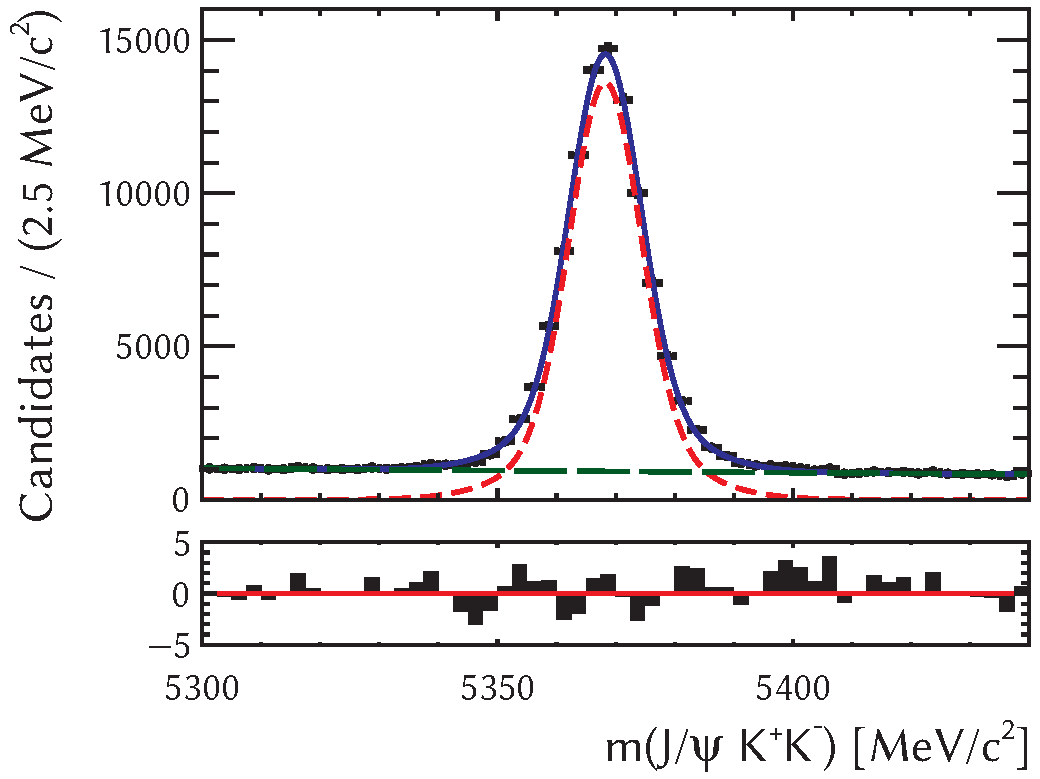
\includegraphics[width=\textwidth]{graphics/analysis/JpsiKKMass_DG_bkgSub_lin_resid}
    \caption{}
    \label{fig:JpsiKKMass_I2_lin}
  \end{subfigure}%
  \hfill%
  \begin{subfigure}{0.49\textwidth}
    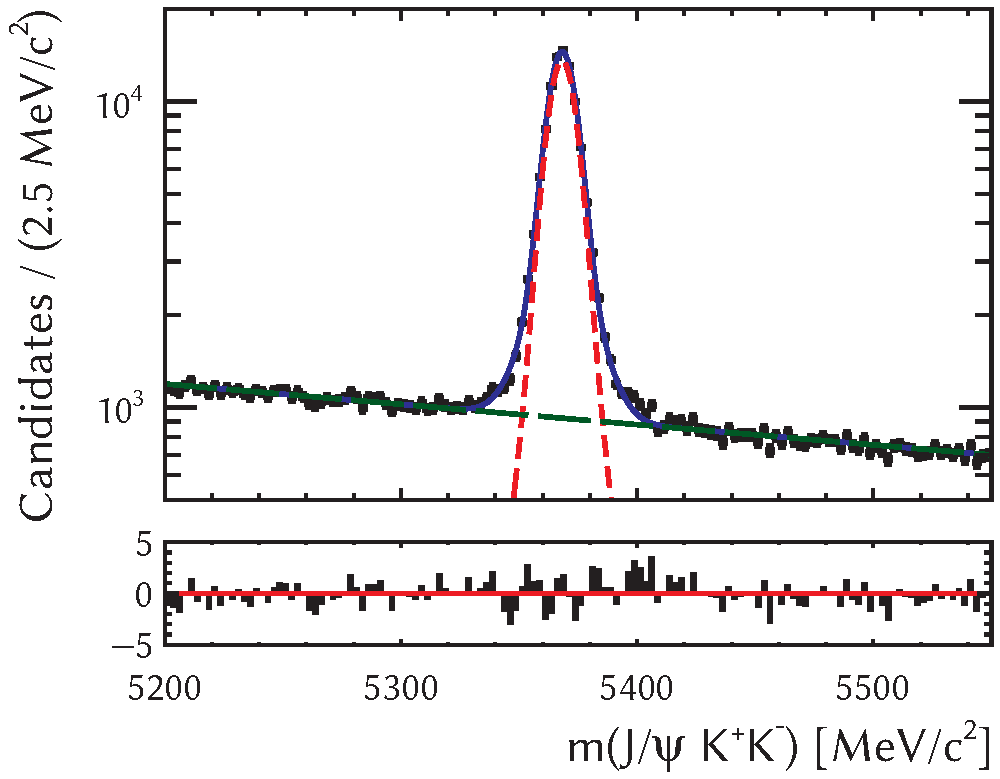
\includegraphics[width=\textwidth]{graphics/analysis/JpsiKKMass_DG_bkgSub_log_resid}
    \caption{}
    \label{fig:JpsiKKMass_I2_log}
  \end{subfigure}%
  \caption{Distribution of \BstoJpsiKK{} decay candidates in $\JpsiKK$ mass after subtracting resonant backgrounds in
           (a) the signal mass range and
           (b) the full mass range on a logarithmic vertical scale.
           The black points show the distribution of the data and the blue, solid line shows a model that was fitted to the data.
           The model is the sum of two Gaussian shapes for the signal (shown by the red, short-dashed line)
           and an exponential shape for combinatorial background (shown by the green, long-dashed line).}
  \label{fig:JpsiKKMass_DG_bkgSub}
\end{figure}

\begin{figure}[tbp]
  \centering
  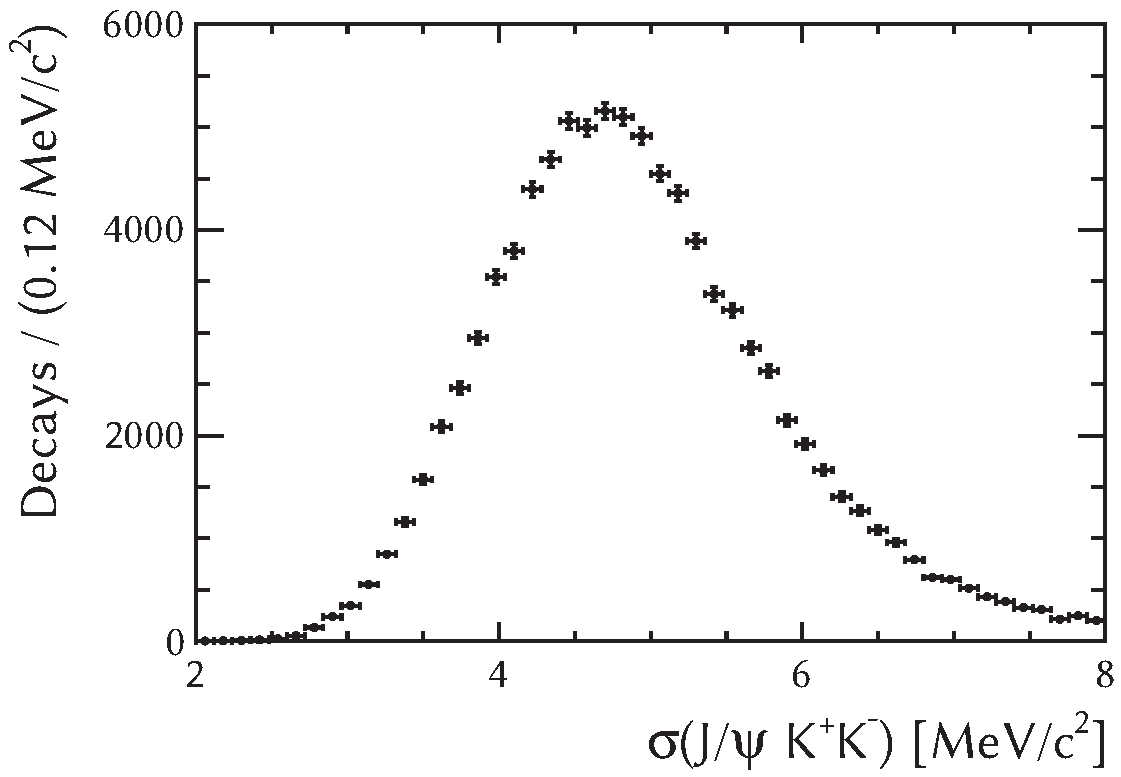
\includegraphics[width=0.5\textwidth]{graphics/analysis/JpsiKKMassErr}
  \caption{Distribution of \BstoJpsiKK{} signal decays in the estimated $\JpsiKK$-mass uncertainty.}
  \label{fig:JpsiKKMassErr}
\end{figure}

To address these issues, the double-Gaussian signal model is replaced by a more sophisticated model for the mass resolution.
Figure~\ref{fig:JpsiKKMassErr} shows the distribution of the estimated uncertainty in the $\JpsiKK$-mass measurement for each decay. This
distribution does not feature a structure with two sharp peaks, as would be expected for a double-Gaussian mass model, but is instead described
by one broad peak. To describe the resulting mass distribution a double-sided Hypatia function with a symmetric core~\cite{Santos:2013gra} is
used, which is designed to describe the effects of an experimental resolution that is different for each decay candidate.

The Hypatia function is defined by
\begin{subequations}
\begin{equation}
  I(m) \equiv
  \begin{cases}
    \left[(m-\mu)^{2} + \delta^{2}\right]^{\frac{1}{2} \lambda - \frac{1}{4}}
          \!\!\!\!& K_{\lambda - \frac{1}{2}}\big(\alpha \sqrt{(m-\mu)^2 + \delta^2}\big) \\
          &\text{if}\ \ -a_L\,\sigma < m - \mu < +a_R\,\sigma \\
    \frac{A_L}{(B_L - m+\mu)^{n_L}} &\text{if}\ \ m - \mu < -a_L\,\sigma \\
    \frac{A_R}{(B_R + m-\mu)^{n_R}} &\text{if}\ \ m - \mu > +a_R\,\sigma
  \end{cases}
\end{equation}
with
\begin{equation}
  \alpha\equiv\frac{1}{\sigma}\sqrt{\frac{\zeta\, K_{\lambda+1}(\zeta)}{K_\lambda(\zeta)}}
  \qquad\text{and}\qquad
  \delta\equiv\sigma\sqrt{\frac{\zeta\,K_\lambda(\zeta)}{K_{\lambda+1}(\zeta)}} \ ,
\end{equation}
\end{subequations}
where $m$ is the mass variable and $K_{\nu}(z)$ the modified Bessel function of the second kind. The parameter $\mu$ controls the position
of the mass peak, $\sigma$ controls the width of its core, and $\lambda$ and $\zeta$ control the shape of its core. The double-sided
Hypatia function has an enhanced tail on both the left and the right side of the mass peak, the positions and shapes of which are
controlled by the parameters $a_{L/R}$ and $n_{L/R}$, respectively. The parameters $A_{L/R}$ and $B_{L/R}$ are obtained by imposing
continuity and differentiability at the points of transition between the core of the function and its tails.

The Hypatia parameters $\lambda$\textapprox\tm2.5, 0\textlt$\zeta$\textlt0.5, $a_{L/R}$\textapprox2.5, and 0\textlt$n_{L/R}$\textlt3 are
determined from simulated \BstoJpsiphi{} signal decays. Only the mean ($\mu$\textapprox5368\unitsp\MeV) and the width
($\sigma$\textapprox8\unitsp\MeV) of the core are determined in a fit to the real data. Consequently, the number of free parameters in the
Hypatia model is smaller than in the double-Gaussian model, for which the mean, the two widths, and the relative contribution of the two
functions were free parameters.

The result of a fit with the Hypatia signal model and an exponential shape for the combinatorial background is shown in
Figure~\ref{fig:JpsiKKMass_I2_bkgSub}. The improvement with the Hypatia model can be seen from the residuals, which have become smaller in
the signal region and are more symmetrically distributed around zero in comparison to Figure~\ref{fig:JpsiKKMass_DG_bkgSub}.

\begin{figure}[tbp]
  \centering
  \begin{subfigure}{0.49\textwidth}
    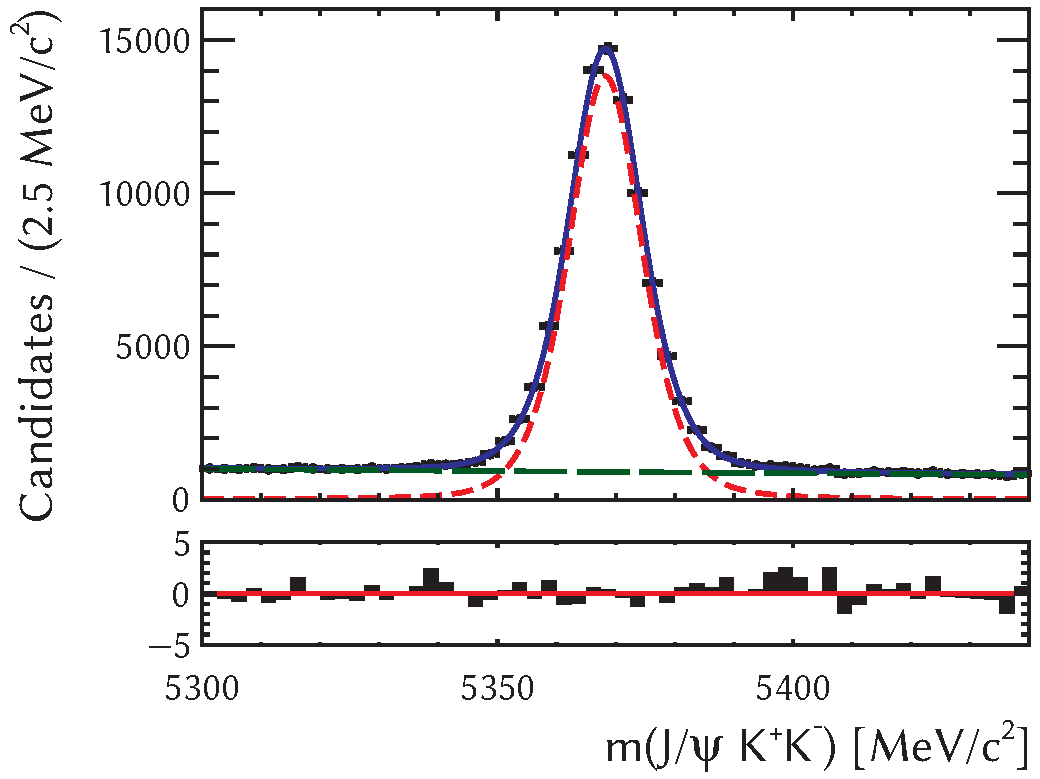
\includegraphics[width=\textwidth]{graphics/analysis/JpsiKKMass_I2_bkgSub_lin_resid}
    \caption{}
    \label{fig:JpsiKKMass_I2_bkgSub_lin}
  \end{subfigure}%
  \hfill%
  \begin{subfigure}{0.49\textwidth}
    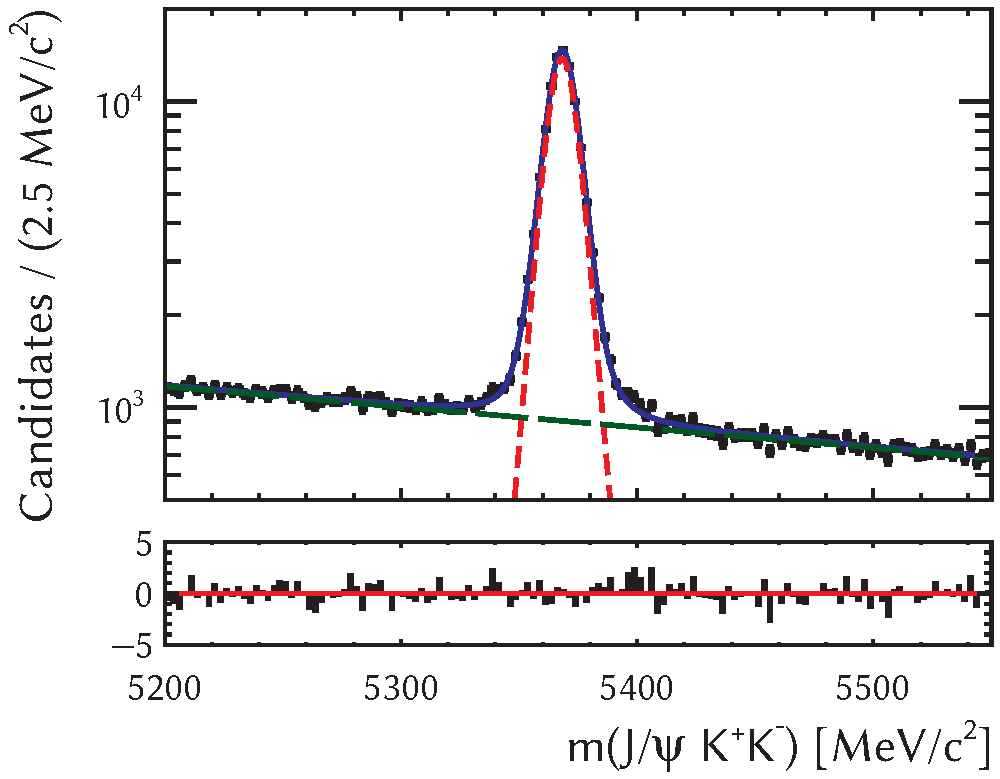
\includegraphics[width=\textwidth]{graphics/analysis/JpsiKKMass_I2_bkgSub_log_resid}
    \caption{}
    \label{fig:JpsiKKMass_I2_bkgSub_log}
  \end{subfigure}%
  \caption{Distribution of \BstoJpsiKK{} decay candidates in $\JpsiKK$ mass after subtracting resonant backgrounds in
           (a) the signal mass range and
           (b) the full mass range on a logarithmic vertical scale.
           The black points show the distribution of the data and the blue, solid line shows a model that was fitted to the data.
           The model is the sum of an Hypatia shape for the signal (shown by the red, short-dashed line)
           and an exponential shape for combinatorial background (shown by the green, long-dashed line).}
  \label{fig:JpsiKKMass_I2_bkgSub}
\end{figure}

Studies of the $\JpsiKK$-mass shape of signal decays have shown that it depends on the $\KK$ invariant mass. Therefore, the parameters of
the mass model are determined separately in the $\KK$-mass bins that are also used in the final time and angular model to determine the
trend in the difference between the $\Jpsiphi$ and $\KK$ S-wave phases (see Section~\ref{subsec:pheno_equations_symmetry}). Combinatorial
background is subtracted separately for each bin.

The $\KK$-mass bins are defined in Table~\ref{tab:KKBins}. In addition to the binning, the table also lists the final numbers of signal and
combinatorial-background decays and the weighted-likelihood correction factors (see Section~\ref{subsec:ana_fit_weights}) for each bin.

\begin{table}[p]
  \centering
  \caption{Definition of the bins in $\KK$ invariant mass.}
  \label{tab:KKBins}
  \begin{tabular}{cccccc}
    \hline
    bin  &  range [\MeV]          &  signal [\tenpow{3}]  &  comb. bkg. [\tenpow{3}]  &  $\alpha_{2011}$  &  $\alpha_{2012}$  \\
    \hline
    1    &  \phantom{0}990--1008  &  \phantom{0}2         &  23                          &  0.42          &  0.39             \\
    2    &  1008--1016            &  10                   &  15                          &  0.79          &  0.76             \\
    3    &  1016--1020            &  35                   &  11                          &  0.94          &  0.93             \\
    4    &  1020--1024            &  28                   &  12                          &  0.92          &  0.92             \\
    5    &  1024--1032            &  13                   &  19                          &  0.77          &  0.77             \\
    6    &  1032--1050            &  \phantom{0}8         &  46                          &  0.51          &  0.51             \\
    \hline
  \end{tabular}
\end{table}

\begin{table}[p]
  \centering
  \caption{Parameters of the $\JpsiKK$-mass model that is used for background subtraction.}
  \label{tab:JpsiKKMassPars}
  \begin{tabular}{ccc}
    \hline
    par.                      &  value            &  stat. uncert.  \\
                              &  [\MeV]           &  [\MeV]         \\
    \hline
    $\mu_1$                   &  5368.47          &  0.25           \\
    $\mu_2$                   &  5367.79          &  0.09           \\
    $\mu_3$                   &  5367.93          &  0.04           \\
    $\mu_4$                   &  5368.65          &  0.05           \\
    $\mu_5$                   &  5368.69          &  0.08           \\
    $\mu_6$                   &  5368.39          &  0.13           \\
    $\sigma_{1,\mathrm{b}}$   &  \phantom{0}8.9   &  0.4            \\
    $\sigma_{2,\mathrm{b}}$   &  \phantom{0}8.23  &  0.11           \\
    $\sigma_{3,\mathrm{b}}$   &  \phantom{0}7.98  &  0.05           \\
    $\sigma_{4,\mathrm{b}}$   &  \phantom{0}7.87  &  0.05           \\
    $\sigma_{5,\mathrm{b}}$   &  \phantom{0}8.40  &  0.10           \\
    $\sigma_{6,\mathrm{b}}$   &  \phantom{0}8.90  &  0.18           \\
    $\sigma_{1,\mathrm{nb}}$  &  14.7             &  3.4            \\
    $\sigma_{2,\mathrm{nb}}$  &  \phantom{0}6.2   &  0.9            \\
    $\sigma_{3,\mathrm{nb}}$  &  \phantom{0}7.0   &  0.4            \\
    $\sigma_{4,\mathrm{nb}}$  &  \phantom{0}7.0   &  0.5            \\
    $\sigma_{5,\mathrm{nb}}$  &  \phantom{0}7.1   &  0.9            \\
    $\sigma_{6,\mathrm{nb}}$  &  \phantom{0}7.6   &  1.8            \\
    \hline
  \end{tabular}%
  \hspace*{15pt}%
  \begin{tabular}{ccc}
    \hline
    par.                         &  value            &  stat. uncert.  \\
     &  [$c$\textsuperscript{2}/MeV]  &  [$c$\textsuperscript{2}/MeV]  \\
    \hline
    $\gamma_{\mathrm{b},2011}$   &  0.00176  &  0.00006  \\
    $\gamma_{\mathrm{b},2012}$   &  0.00153  &  0.00003  \\
    $\gamma_{\mathrm{nb},2011}$  &  0.00032  &  0.00024  \\
    $\gamma_{\mathrm{nb},2012}$  &  0.00054  &  0.00015  \\
    \hline
    & & \\ & & \\ & & \\ & & \\ & & \\ & & \\ & & \\ & & \\ & & \\ & & \\ & & \\ & & \\ & & \\ & & \\
  \end{tabular}
\end{table}

There is no evidence for the $\JpsiKK$-mass distribution of the background to depend on the $\KK$ mass, but it does depend on two other
variables in the data. The background distribution is found to be different for the 2011 and 2012 run periods and for decay candidates that
are selected by the biased HLT2 trigger and candidates that are exclusively selected by the unbiased HLT2 trigger. Because these two
variables are used in the measurement and implementation of the decay-time efficiency function (see Section~\ref{subsec:ana_time_acc}),
background subtraction is also performed separately in the four categories associated to these variables. In addition, the  width of the
signal peak is determined separately for HLT2-biased and not-HLT2-biased candidates.

The final parameters of the $\JpsiKK$-mass model that were determined from the real data are listed in Table~\ref{tab:JpsiKKMassPars},
where the exponential function for the background mass distribution is described by $e^{-\gamma m}$. The number of signal decays determined
with this model is 96 thousand and the number of combinatorial-background decays 127 thousand.

To check if the decay time and angles are not correlated with the $\JpsiKK$ mass, the mass distribution is plotted for different bins in
time and angles. A problem appears in $\cthetal$, for which the mass distributions are shown in the bins $|\cthetal|$\textlt0.25,
0.25\textle$|\cthetal|$\textlt0.7, and $|\cthetal|$\textge0.7 in Figure~\ref{fig:JpsiKKMass_I2_bkgSub_ctl}. In all three cases the nominal
mass model from Figure~\ref{fig:JpsiKKMass_I2_bkgSub} is shown.
\begin{figure}[tbp]
  \centering
  \begin{subfigure}{0.49\textwidth}
    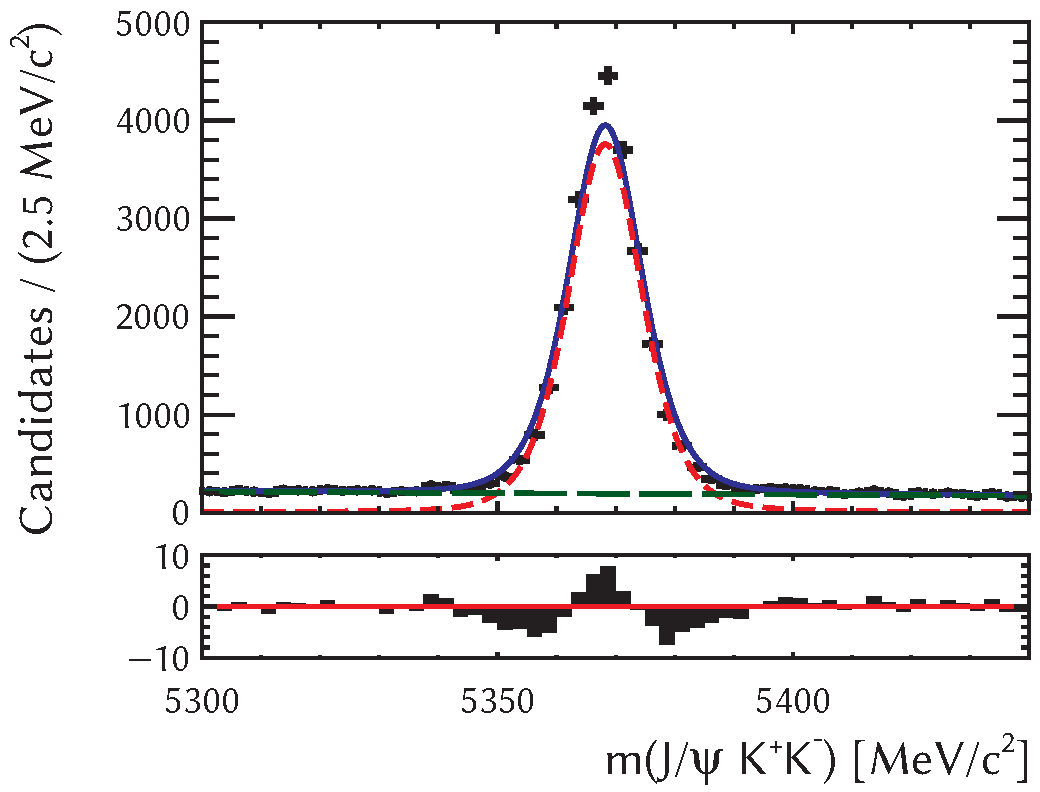
\includegraphics[width=\textwidth]{graphics/analysis/JpsiKKMass_I2_bkgSub_ctl2_lin_resid}
    \caption{}
    \label{fig:JpsiKKMass_I2_bkgSub_ctl2_lin}
  \end{subfigure}%
  \hfill%
  \begin{subfigure}{0.49\textwidth}
    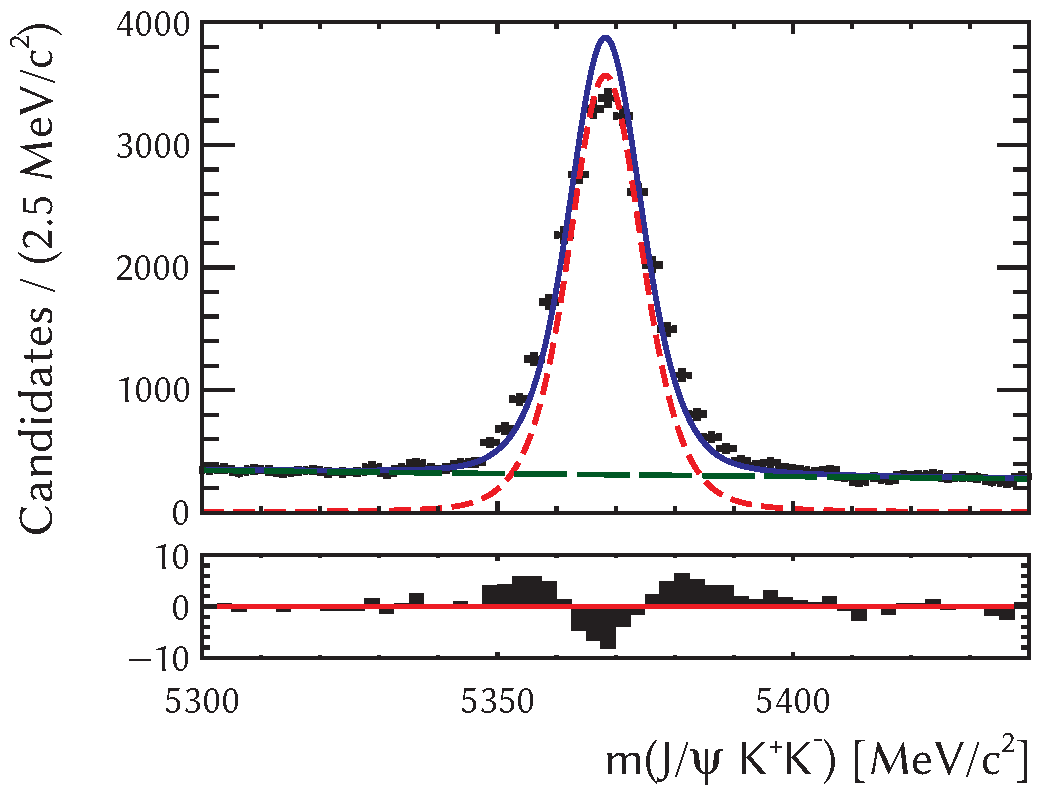
\includegraphics[width=\textwidth]{graphics/analysis/JpsiKKMass_I2_bkgSub_ctl04_lin_resid}
    \caption{}
    \label{fig:JpsiKKMass_I2_bkgSub_ctl04_lin}
  \end{subfigure}

  \vspace*{0.02\textwidth}
  \begin{subfigure}{0.49\textwidth}
    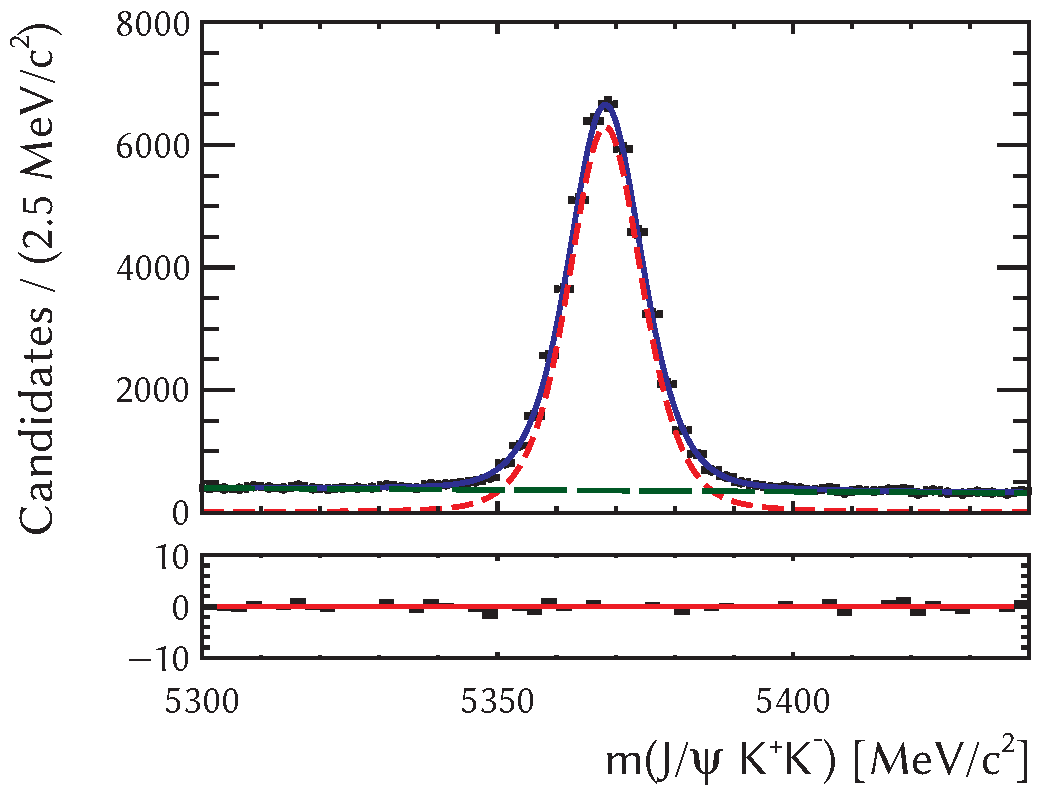
\includegraphics[width=\textwidth]{graphics/analysis/JpsiKKMass_I2_bkgSub_ctl13_lin_resid}
    \caption{}
    \label{fig:JpsiKKMass_I2_bkgSub_ctl13}
  \end{subfigure}%
  \caption{Distribution of \BstoJpsiKK{} decay candidates in $\JpsiKK$ mass after subtracting resonant backgrounds in bins of $\cthetal$,
           where the shape of the model is set to the nominal shape from Figure~\ref{fig:JpsiKKMass_I2_bkgSub}.
           (a) $|\cthetal|$\textlt0.25,
           (b) $|\cthetal|$\textge0.7,
           (c) 0.25\textle$|\cthetal|$\textlt0.7.}
  \label{fig:JpsiKKMass_I2_bkgSub_ctl}
\end{figure}

\begin{figure}[tbp]
  \centering
  \begin{subfigure}{0.49\textwidth}
    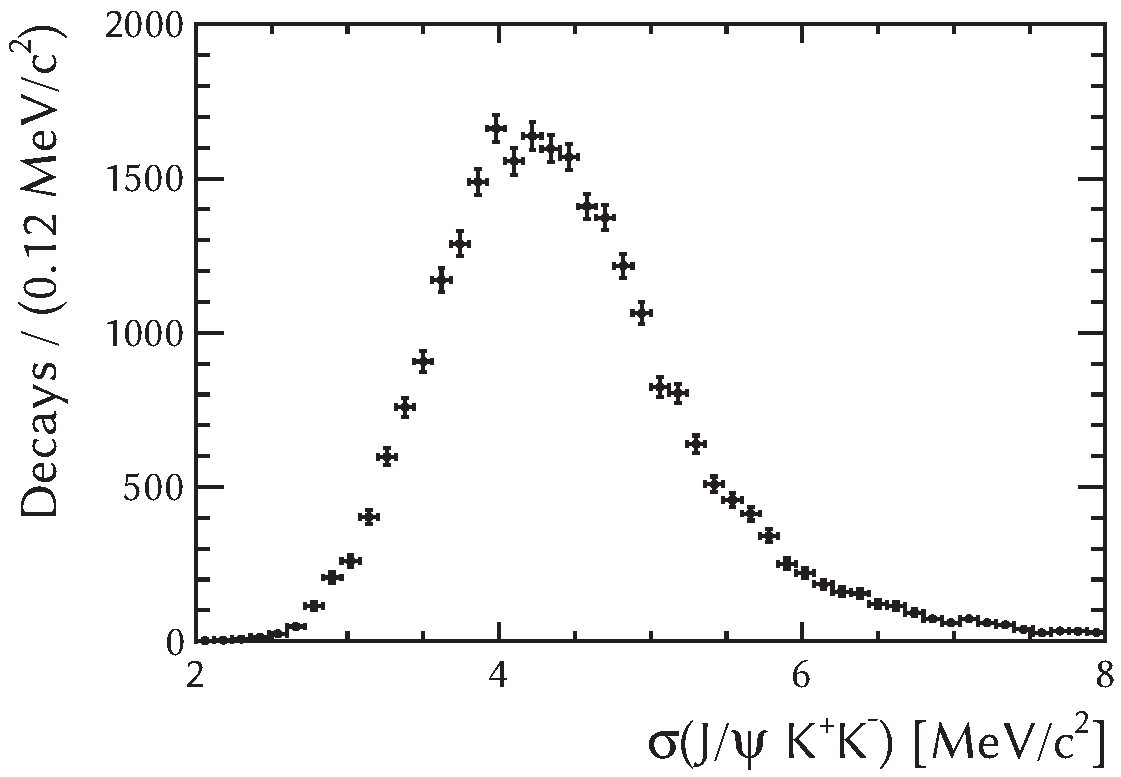
\includegraphics[width=\textwidth]{graphics/analysis/JpsiKKMassErr_left}
    \caption{}
    \label{fig:JpsiKKMassErr_left}
  \end{subfigure}%
  \hfill%
  \begin{subfigure}{0.49\textwidth}
    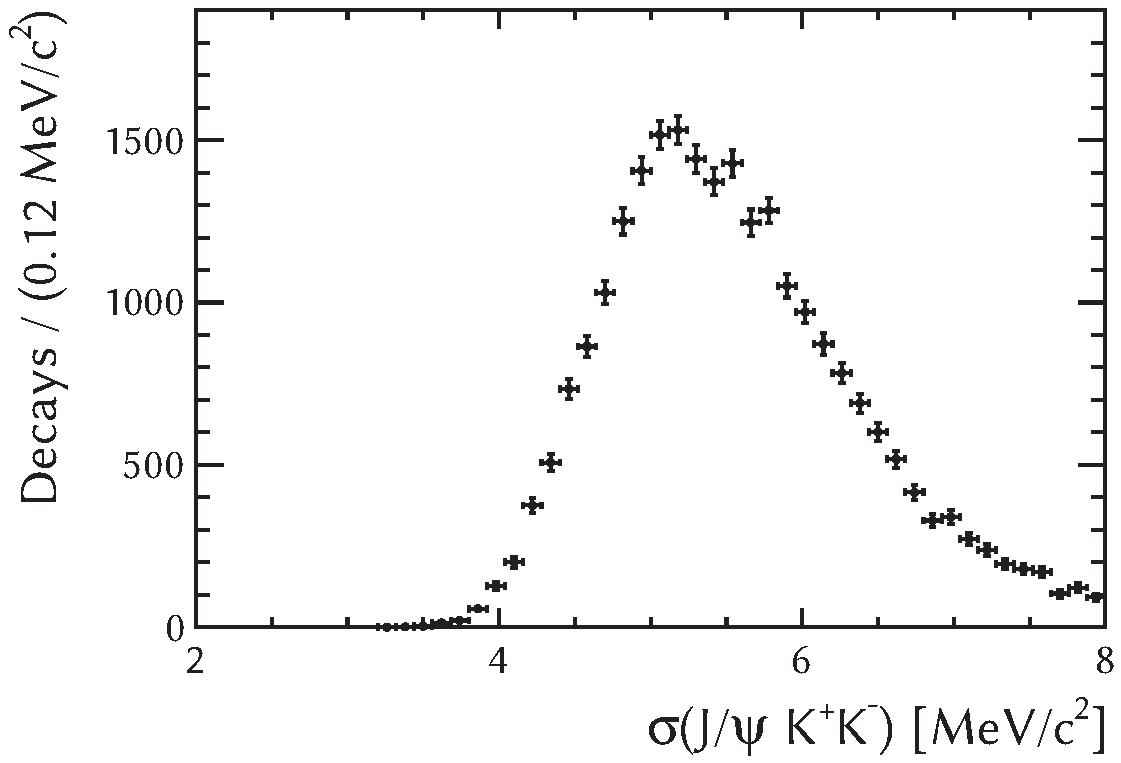
\includegraphics[width=\textwidth]{graphics/analysis/JpsiKKMassErr_right}
    \caption{}
    \label{fig:JpsiKKMassErr_right}
  \end{subfigure}

  \vspace*{0.02\textwidth}
  \begin{subfigure}{0.49\textwidth}
    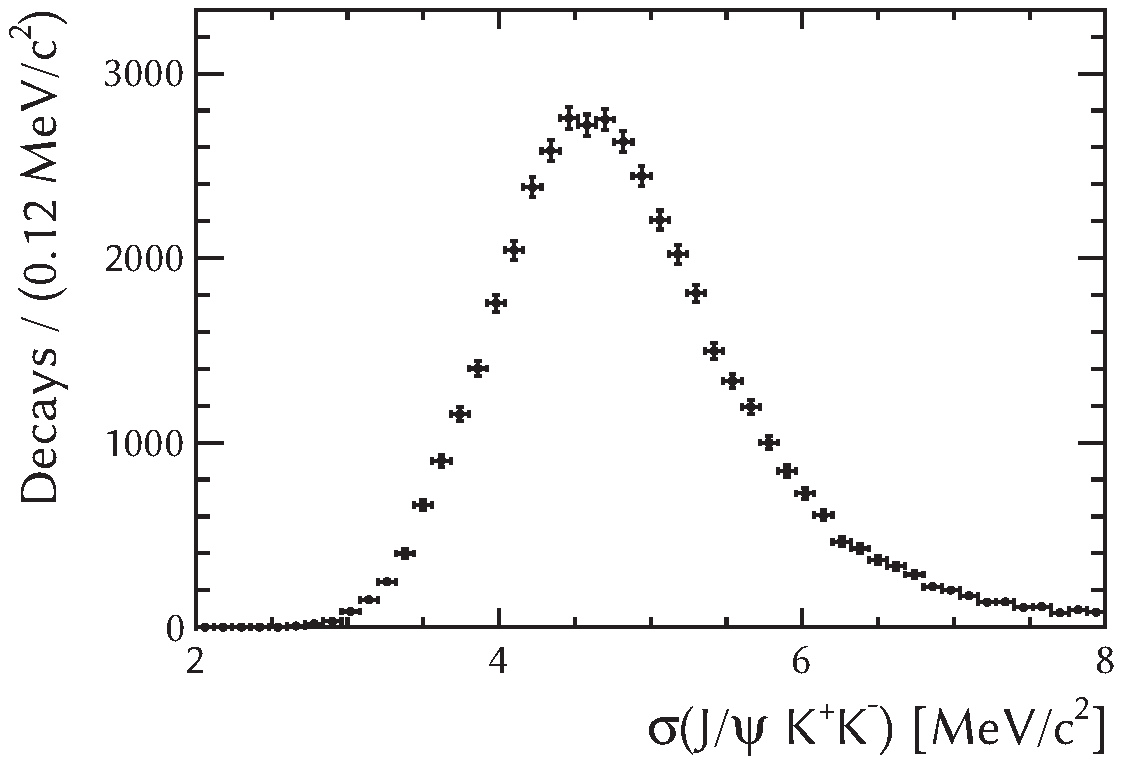
\includegraphics[width=\textwidth]{graphics/analysis/JpsiKKMassErr_middle}
    \caption{}
    \label{fig:JpsiKKMassErr_middle}
  \end{subfigure}%
  \caption{Distribution of \BstoJpsiKK{} signal decays in the estimated $\JpsiKK$-mass uncertainty in bins of $\cthetal$.
           (a) $|\cthetal|$\textlt0.25,
           (b) $|\cthetal|$\textge0.7,
           (c) 0.25\textle$|\cthetal|$\textlt0.7.}
  \label{fig:JpsiKKMassErr_ctlBins}
\end{figure}

\begin{figure}[p]
  \centering
  \begin{subfigure}{0.49\textwidth}
    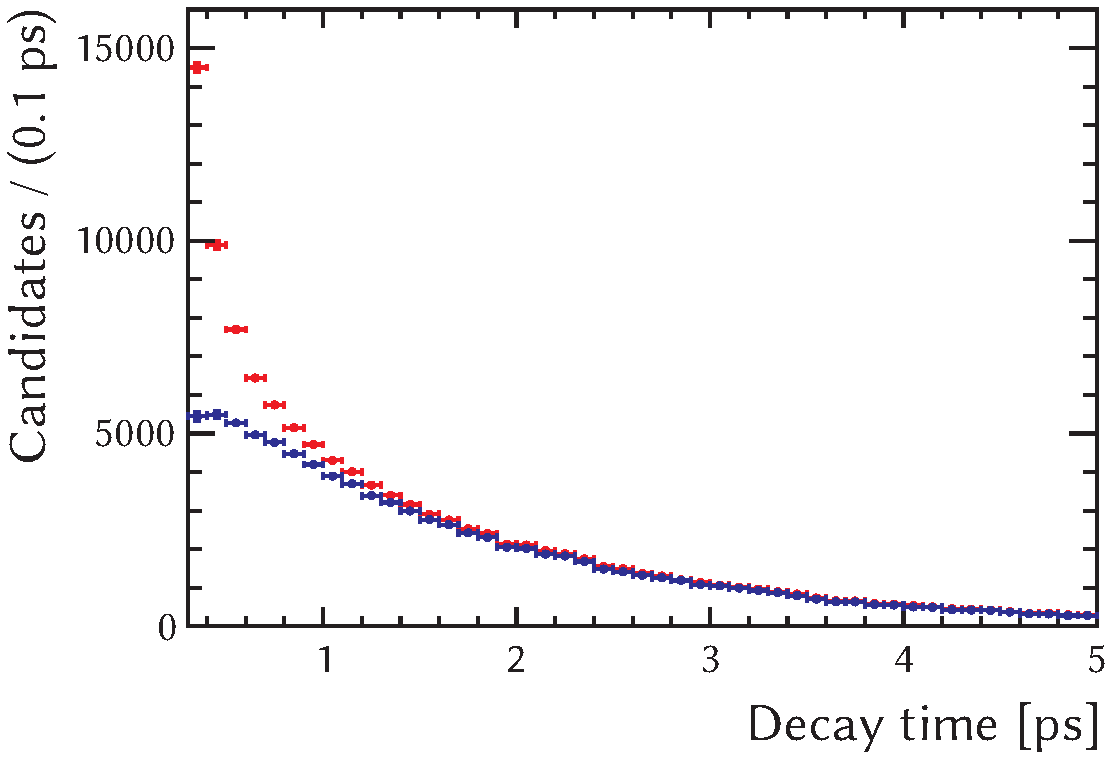
\includegraphics[width=\textwidth]{graphics/analysis/time_bkgSub}
    \caption{}
    \label{fig:timeBkgSub}
  \end{subfigure}%
  \hfill%
  \begin{subfigure}{0.49\textwidth}
    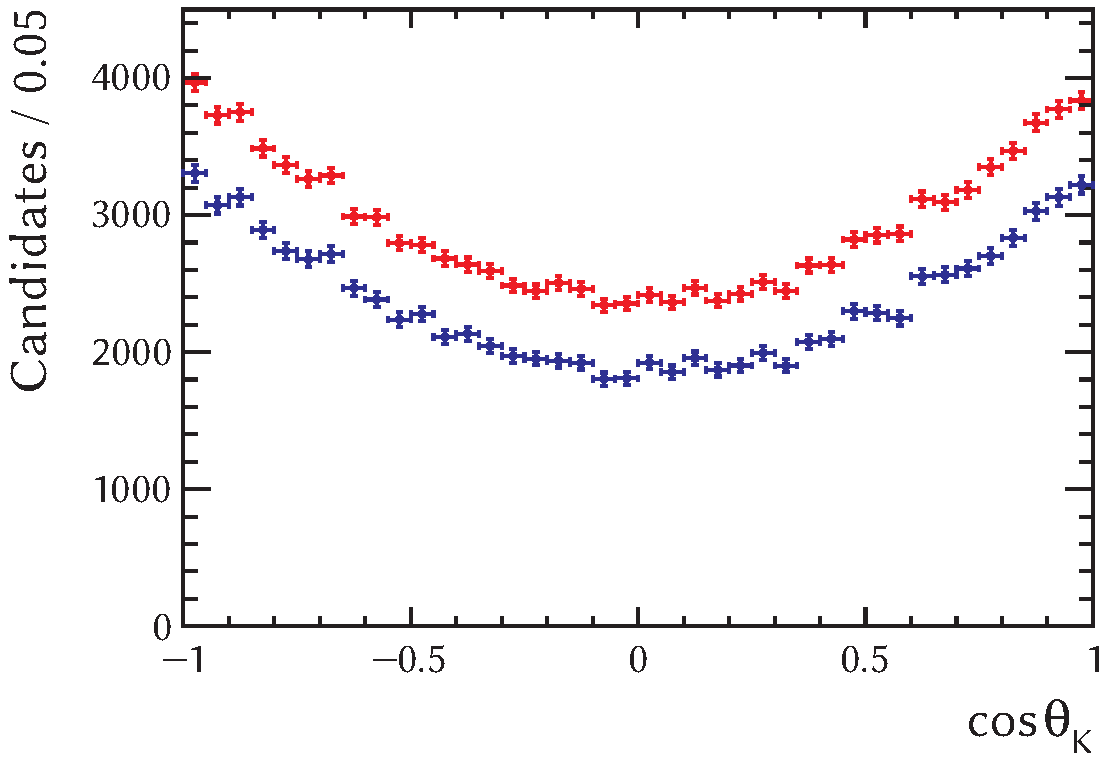
\includegraphics[width=\textwidth]{graphics/analysis/ctk_bkgSub}
    \caption{}
    \label{fig:ctkBkgSub}
  \end{subfigure}

  \vspace*{0.02\textwidth}
  \begin{subfigure}{0.49\textwidth}
    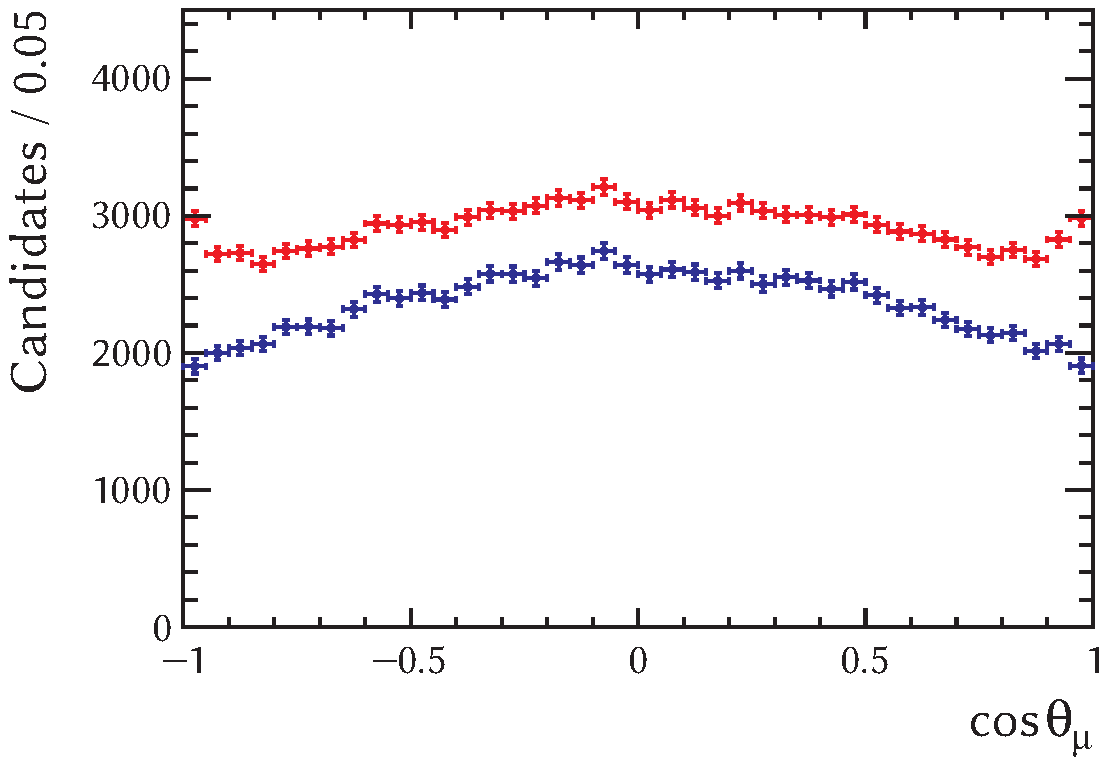
\includegraphics[width=\textwidth]{graphics/analysis/ctl_bkgSub}
    \caption{}
    \label{fig:ctlBkgSub}
  \end{subfigure}%
  \hfill%
  \begin{subfigure}{0.49\textwidth}
    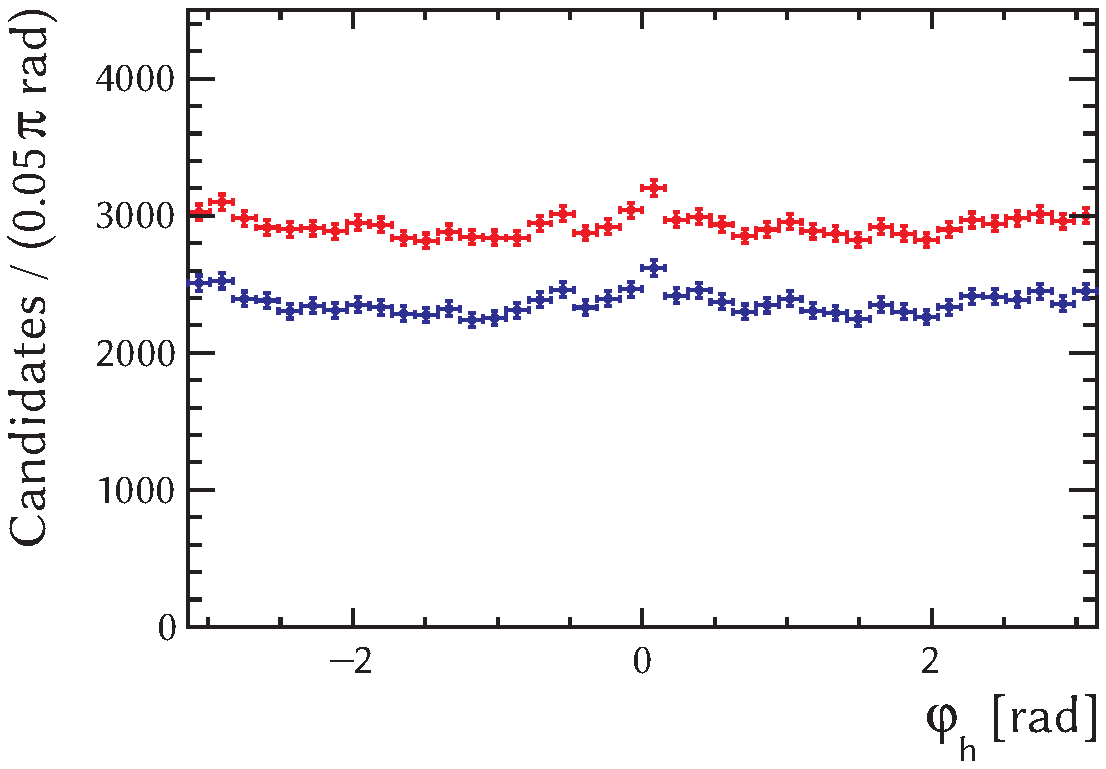
\includegraphics[width=\textwidth]{graphics/analysis/phi_bkgSub}
    \caption{}
    \label{fig:phiBkgSub}
  \end{subfigure}

  \vspace*{0.02\textwidth}
  \begin{subfigure}{0.49\textwidth}
    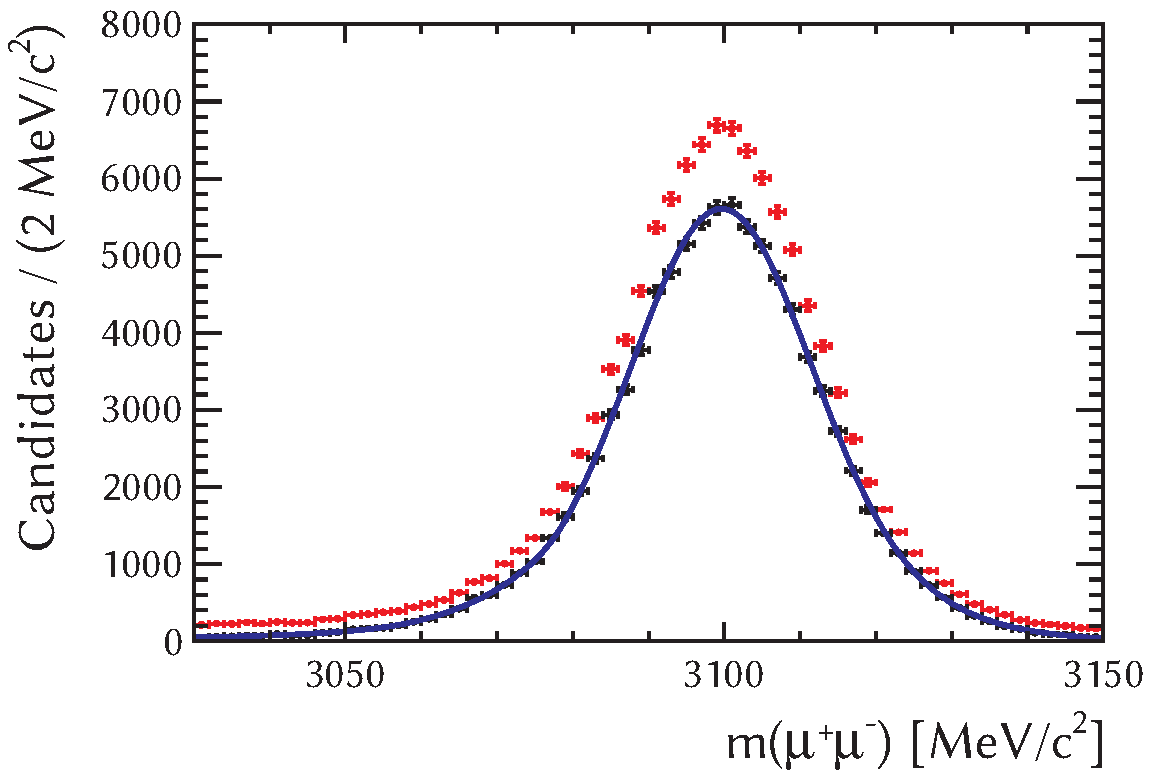
\includegraphics[width=\textwidth]{graphics/analysis/mumuMass_bkgSub_lin}
    \caption{}
    \label{fig:mumuMassBkgSub}
  \end{subfigure}%
  \hfill%
  \begin{subfigure}{0.49\textwidth}
    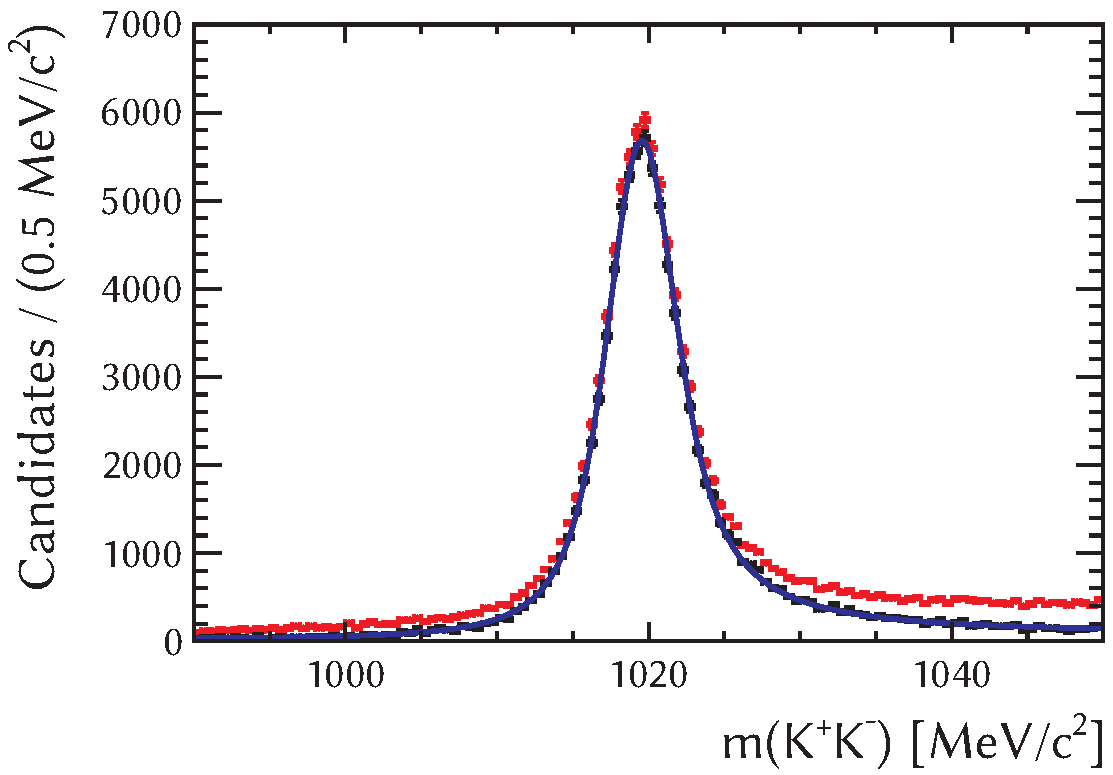
\includegraphics[width=\textwidth]{graphics/analysis/KKMass_bkgSub_lin}
    \caption{}
    \label{fig:KKMassBkgSub}
  \end{subfigure}%

  \caption{Distributions of \BstoJpsiKK{} decay candidates before (red) and after (blue) background subtraction
           in (a) decay time, (b) $\cthetaK$, (c) $\cthetal$, (d) $\phihel$, (e) $\mumu$ mass, and (f) $\KK$ mass.
           The distributions before background subtraction are for decay candidates
           in a $\JpsiKK$-mass window of 60\unitsp\MeV{} around the $\Bs$ mass.}
  \label{fig:obsBkgSub}
\end{figure}

From Figure~\ref{fig:JpsiKKMass_I2_bkgSub_ctl} it is clear that the $\JpsiKK$-mass resolution for the signal depends on the value of
$\cthetal$. This is also supported by Figure~\ref{fig:JpsiKKMassErr_ctlBins}, which shows that the distribution of the estimated $\JpsiKK$-mass
uncertainty varies for the three $\cthetal$ regions. Formally this means that the procedure of background subtraction does not work for the
$\cthetal$ distribution. The impact of this effect is studied by subtracting the background with the different mass models obtained in the
$\cthetal$ bins and a corresponding systematic uncertainty is evaluated (see Section~\ref{sec:result_syst}).

Figure~\ref{fig:obsBkgSub} shows the distributions of decay time, decay angles, $\mumu$ invariant mass, and $\KK$ invariant mass before and
after background subtraction. The distributions before background subtraction are only shown for a $\JpsiKK$-mass window of 60\unitsp\MeV{}
around the $\Bs$ mass.

From the decay-time distribution in Figure~\ref{fig:timeBkgSub} it can be seen that most background candidates have a small decay time.
Notice that the decay-time range in this plot starts at 0.3\unitsp{}ps. Even though the first of the oscillations in the decay time
distribution of the signal is lost, this requirement improves the measurement, because it removes a significant amount of background, as
shown in Section~\ref{subsec:ana_bkgSub_sel}.

The model that was fitted to the $\mumu$-mass distribution in Figure~\ref{fig:mumuMassBkgSub} consists of the sum of two Gaussian shapes,
with a polynomial that describes the enhanced tail on the left of the mass peak, which is due to photon radiation after the decay of the
$\Jpsi$. The model for the $\KK$-mass distribution consists of a relativistic Breit-Wigner shape for the $\Jpsiphi$ contribution and a
polynomial for the $\KK$ S-wave. From this fit, an S-wave fraction of approximately 5\% is found.

Note that the models for the $\mumu$ and $\KK$ mass that were used to fit the distributions in Figures~\ref{fig:mumuMassBkgSub} and
\ref{fig:KKMassBkgSub} are not used in the decay model, except for the latter in the calculation of the $\CSP$ factors. The distributions
of time and angles in Figures~\ref{fig:timeBkgSub}--d are described by the model discussed in Chapter~\ref{chap:pheno} with the
experimental effects that will be discussed in the following sections.

\section{Decay Time}
\label{sec:ana_time}

The theoretical model of the decay time of \BstoJpsiKK{} decays is distorted by two experimental effects; the uncertainty in the time
measurement (\emph{resolution}) and the efficiency of the measurement (\emph{acceptance}) as a function of time. As discussed in
Section~\ref{subsec:intro_LHCb_Jpsiphi}, the resolution is roughly 0.05\unitsp{}ps. The resolution model is presented in
Section~\ref{subsec:ana_time_res}. The decay-time measurement is affected by non-trivial acceptance effects from both the trigger and
reconstruction processes, which will be discussed in Section~\ref{subsec:ana_time_acc}.


%%%%%%%%%%%%%%%%%%%%%%%%%%%
\subsection{Resolution}
\label{subsec:ana_time_res}
%%%%%%%%%%%%%%%%%%%%%%%%%%%

The uncertainty in the decay-time measurement causes a difference between the measured decay time and the true decay time. This difference
is a random variable and the resulting measured time distribution is a smeared version of the underlying true distribution. For the
oscillatory $\cDms$ and $\sDms$ functions in the differential decay rate this smearing causes a decrease, or \emph{dilution}, of the
oscillation amplitude. As described in Section~\ref{subsec:pheno_equations_approx}, the main sensitivity for the CP-violation parameters
originates from the oscillation terms and hence a diluted oscillation amplitude reduces the statistical precision of the estimates for
these parameters.

For each decay the decay-time uncertainty is estimated by propagating the uncertainties in the positions of the primary and secondary
vertices and particle momenta, as discussed in Section~\ref{subsec:intro_LHCb_Jpsiphi}. The distribution of this estimate ($\sigmat$) is
shown in Figure~\ref{fig:sigmat}. For each decay, the probability for the measured decay time to deviate by a given amount from the true
decay time is approximately described by a Gaussian distribution with width $\sigmat$.
\begin{figure}[htbp]
  \centering
  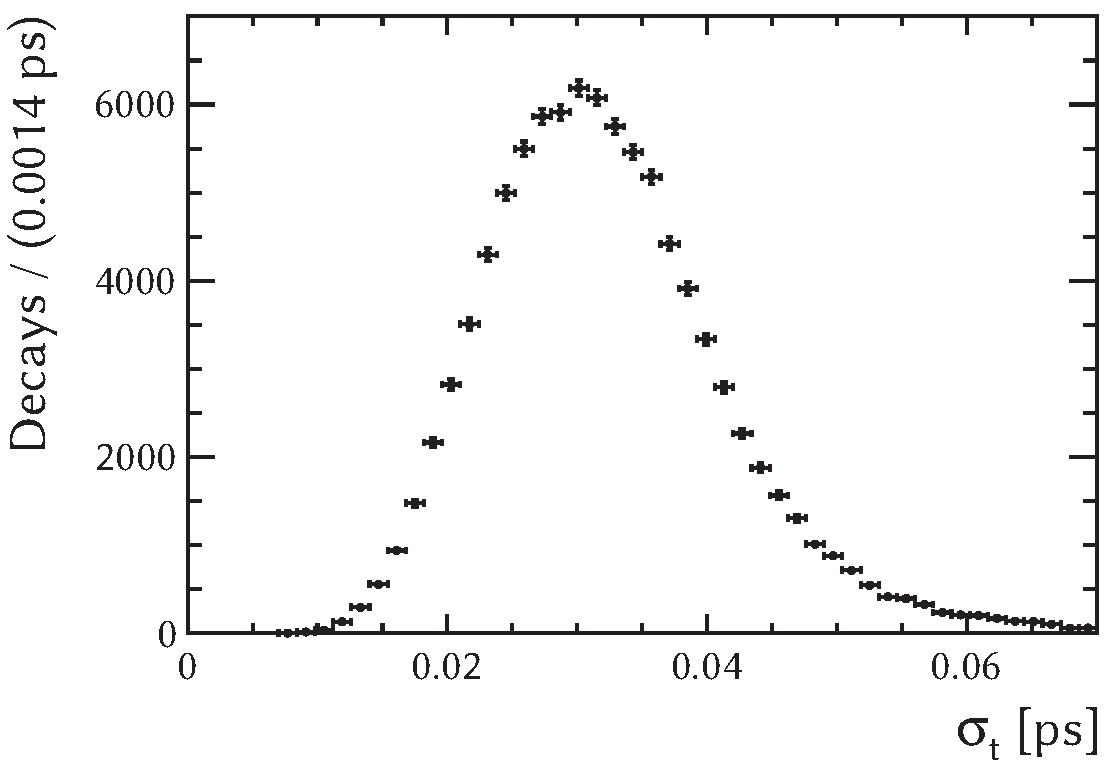
\includegraphics[width=0.5\textwidth]{graphics/analysis/sigmat}
  \caption{Distribution of \BstoJpsiKK{} signal decays in the estimated decay-time uncertainty.}
  \label{fig:sigmat}
\end{figure}

Decay-time resolution is included in the model for the signal decay by convolving the theoretical model with the model for the difference
between the measured time and the true time. This convolution is the integral of the two-dimensional PDF of the true and measured decay
times over all possible values of the former:
\begin{equation}
  P_\text{meas}(t_\text{meas}, \Omega)
    \equiv \int_0^\infty \ud t_\text{true}\, R(t_\text{meas} - t_\text{true}|\sigmat)\, P_\text{true}(t_\text{true}, \Omega)\ ,
\end{equation}
where $R$ is the PDF for the difference between the measured and true times, or the \emph{resolution model}. The resolution model is
conditional on $\sigmat$., i.e. normalized with respect to decay time for each individual value of $\sigmat$.

Although the resolution model is approximated by a Gaussian PDF with width $\sigmat$, a more sophisticated model is required to describe
the resolution in the PDF with sufficient precision. The model is a sum of two Gaussian PDFs with a common, non-zero mean and a width that
depends quadratically on $\sigmat$. The width of the first Gaussian PDF is approximately equal to $\sigmat$, while the width of the second
Gaussian PDF is roughly a factor two larger.

The double-Gaussian model is based on and validated with both simulated \BstoJpsiKK{} decays and prompt background decay candidates. Since
all tracks of prompt background candidates originate from the primary vertex, their ``true'' decay time is equal to zero and the
distribution of measured decay times is essentially the resolution model. Studies of the model and its parameters are described in detail
in references~\cite{Aaij:2015} and \cite{LHCb-ANA-2014-039}. The values of the resolution parameters are fixed in the fit of decay time and
angles. Uncertainties in the parameter values are propagated after the fit and accounted for as systematic uncertainties (see
Section~\ref{sec:result_syst}).


%%%%%%%%%%%%%%%%%%%%%%%%%%%
\subsection{Acceptance}
\label{subsec:ana_time_acc}
%%%%%%%%%%%%%%%%%%%%%%%%%%%

To account for the efficiencies of the decay-candidate reconstruction and selection processes, the PDF is multiplied by an acceptance
function and re-normalized to create a new PDF. The acceptance is is modelled as a product of two functions of decay time and one function
of decay angles. The angular part will be discussed in Section~\ref{sec:ana_angles}. This section describes the two decay-time functions.

\subsubsection{Track-Reconstruction Acceptance}
The first part of the non-trivial acceptance in decay time originates from an inefficiency in the reconstruction of particle tracks. This
efficiency decreases for increasing distance between the track and the proton beams. Since the distance between the primary and secondary
vertex and, therefore, the decay time are correlated with the distance between the four \BstoJpsiKK{} tracks and the beams, the efficiency
also decreases with increasing decay time.

In the measurement presented here the track-reconstruction acceptance is modelled by an exponential function in \emph{true} decay time. The
advantage of this model is that its implementation in the model of the decay-time distribution is straightforward. An exponential function
can be absorbed in the $\eGst$ factor of the differential decay rate (Equation~\ref{eq:angCoefs}):
\begin{equation}
  \eGst \longrightarrow e^{\beta\,t}\,\eGst = e^{-(\Gs-\beta)\,t} \equiv e^{-\Gs^\text{eff}\,t}\ ,
\end{equation}
where $\beta$ is the parameter that quantifies the rate at which the efficiency changes as a function of decay time. The parameter
$\Gs^\text{eff}$\textequiv$\Gs$\textminus$\beta$ can now be included in the model in the place of the parameter $\Gs$.

The parameter $\beta$ has been determined by a combination of studies with real and simulated data~\cite{LHCb-ANA-2014-039}. Because of
changes in the online reconstruction algorithms between the 2011 and 2012 runs and the different proton-collision energies in these
periods, the corresponding values of $\beta$ are evaluated separately: $\beta_\text{2011}$\texteq\mbox{\tm0.0090\textpm0.0022\unitsp\invps}
and $\beta_\text{2012}$\texteq\mbox{\tm0.0124\textpm0.0019\unitsp\invps}. These values have to be compared with
$\Gs$\textapprox0.66\unitsp\invps.

Although there is no sensitivity in the \BstoJpsiKK{} data to the parameters $\Gs$, $\beta_\text{2011}$, and $\beta_\text{2012}$
separately, the value of $\Gs^\text{eff}$ can be determined in the fit of decay time separately for the 2011 and 2012 periods.
Reparameterizing, there is sensitivity for the combinations $\Gs$\textminus$\tfrac{1}{2}(\beta_\text{2011}$\textplus$\beta_\text{2012})$
and $\beta_\text{2012}$\textminus$\beta_\text{2011}$.

To combine the information on the difference between the two $\beta$ values with the externally determined values, the $\beta$ parameters
are varied with constraints in the time and angular fit. These constraints are implemented by adding a parabolic term to the NLL of the
form $\frac{1}{2\hat{\sigma}^2}(\beta-\hat{\beta})^2$ for each parameter, where the external value is denoted by $\hat{\beta}$ and the
external uncertainty by $\hat{\sigma}$. Because these external constraints are much tighter than the constraints from the \BstoJpsiKK{}
data, the values that are estimated in the fit are comparable to the external values:
$\beta_\text{2011}$\texteq\mbox{\tm0.0086\textpm0.0021\unitsp\invps} and
$\beta_\text{2012}$\texteq\mbox{\tm0.0127\textpm0.0018\unitsp\invps}.

There are some limitations to this model of the track-reconstruction acceptance. The model is implemented for true decay time, whereas the
external values of the $\beta$ parameters were evaluated with the measured decay time. In this measurement, this is assumed to be a good
approximation, because the time scale of the variations in the model is much larger than the resolution. That is,
$\beta^{-1}$\textapprox\mbox{\tenpow{2}\unitsp{}ps}\textgg\mbox{0.05\unitsp{}ps}.

Also the model itself is an approximation. As was shown in reference~\cite{LHCb-ANA-2014-039}, the shape of the acceptance is better
described by the function 1\textplus$\beta\,t$\textplus$\beta'\,t^2$ than by $e^{\beta\,t}$\textapprox1\textplus$\beta\,t$. A systematic
uncertainty in the parameter estimates corresponding to the assumption of the shape $e^{\beta\,t}$ is estimated in
Section~\ref{sec:result_syst}.

\subsubsection{Trigger Acceptance}
As described in Section~\ref{subsec:ana_bkgSub_sel}, there are also trigger requirements that introduce non-trivial acceptance effects in
decay time. The shapes of the acceptance functions corresponding to the decay-time biasing trigger categories are determined relative to
the shapes of the unbiased categories, which have a uniform acceptance function.

The shape of the trigger acceptance is described in bins of decay time. For each bin, numbers of decays are counted in the different
trigger categories to determine the relative efficiency in the bin. To also include information on the exponential shape of the decay in
the resulting binned acceptance function, the decay counts are varied in the fit of decay time and angles.

Since originally only the shape of the differential decay rate in time and angles is determined in the fit, additional terms need to be
included in the NLL to count decays in the different trigger categories. For unweighted decays the PDF for the number of decays in a
category would be a Poisson distribution, which is proportional to $\nu^n\,e^{-\nu}$, where $n$ is the observed number of decays and $\nu$
is the parameter for the expected number of decays. This PDF would give an additional NLL term of $\nu$\textminus$n\,\ln\nu$. However,
because each decay candidate is counted with its signal weight, this term is modified to obtain the correct uncertainty on the parameter
$\nu$ from a maximum-likelihood fit.

Instead of only replacing the variable $n$ in the Poissonian NLL term by the sum of the decay-candidate weights, the term is also
multiplied by weight factor:
\begin{equation}
  \frac{\sum w}{\sum w^2}\left( \nu - \ln\nu\,\sum w \right)\ ,
\end{equation}
where $\sum w$ is the sum of the decay weights and $\sum w^2$ the sum of the squared decay weights. This function reaches its minimum at
$\nu$\texteq$\sum w$, so the estimated value for $\nu$ in a maximum-likelihood fit with only this function would be the sum of the decay
weights. The inverse of the second derivative of the function, from which the uncertainty in $\nu$ is estimated, is given by $\sum w^2$
instead of $\sum w$ for an unmodified Poisson term. The former number is equal to the variance that is expected when counting weighted
decay candidates.

\begin{itemize}
  \item describe trigger categories and efficiency parameters
  \item using all categories (6) vs merging categories (4 or 5)
  \item short description of resulting acceptance functions (plots): $\longrightarrow$ Roel
\end{itemize}

%Since only decay candidates that are selected by the HLT2-biased trigger line are used for the fit of decay time and angles, only the
%trigger-acceptance functions for the HLT1-unbiased/HLT2-biased and exclusively-HLT1-biased/HLT2-biased combinations are required.

\begin{figure}[htbp]
  \centering
  \begin{subfigure}{0.49\textwidth}
    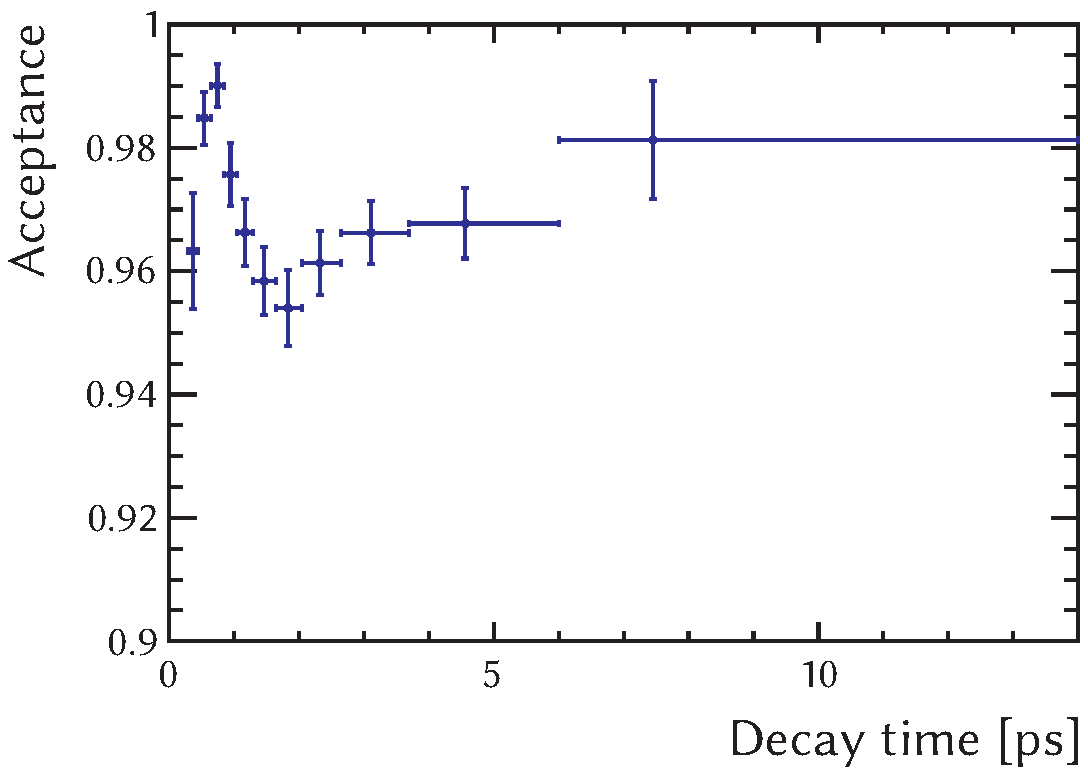
\includegraphics[width=\textwidth]{graphics/analysis/trigTimeAcc_2011_UB}
    \caption{}
    \label{fig:trigAcc_2011_UB}
  \end{subfigure}%
  \hfill%
  \begin{subfigure}{0.49\textwidth}
    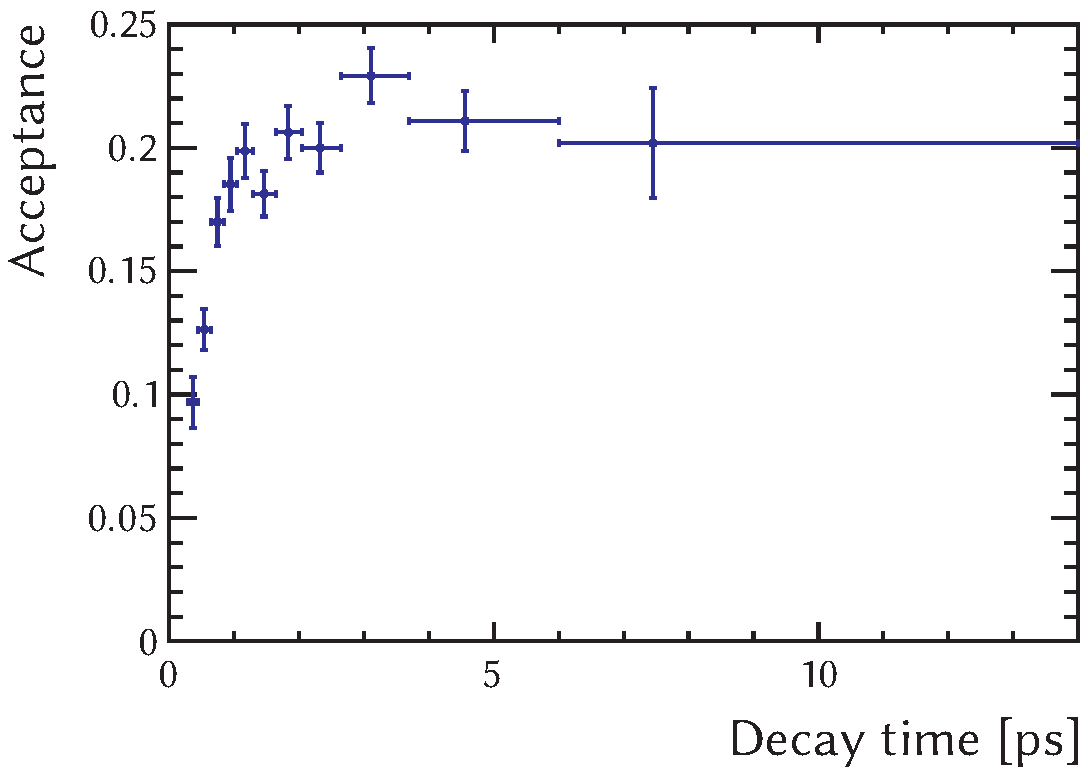
\includegraphics[width=\textwidth]{graphics/analysis/trigTimeAcc_2011_exclB}
    \caption{}
    \label{fig:trigAcc_2011_exclB}
  \end{subfigure}

  \vspace*{0.02\textwidth}
  \begin{subfigure}{0.49\textwidth}
    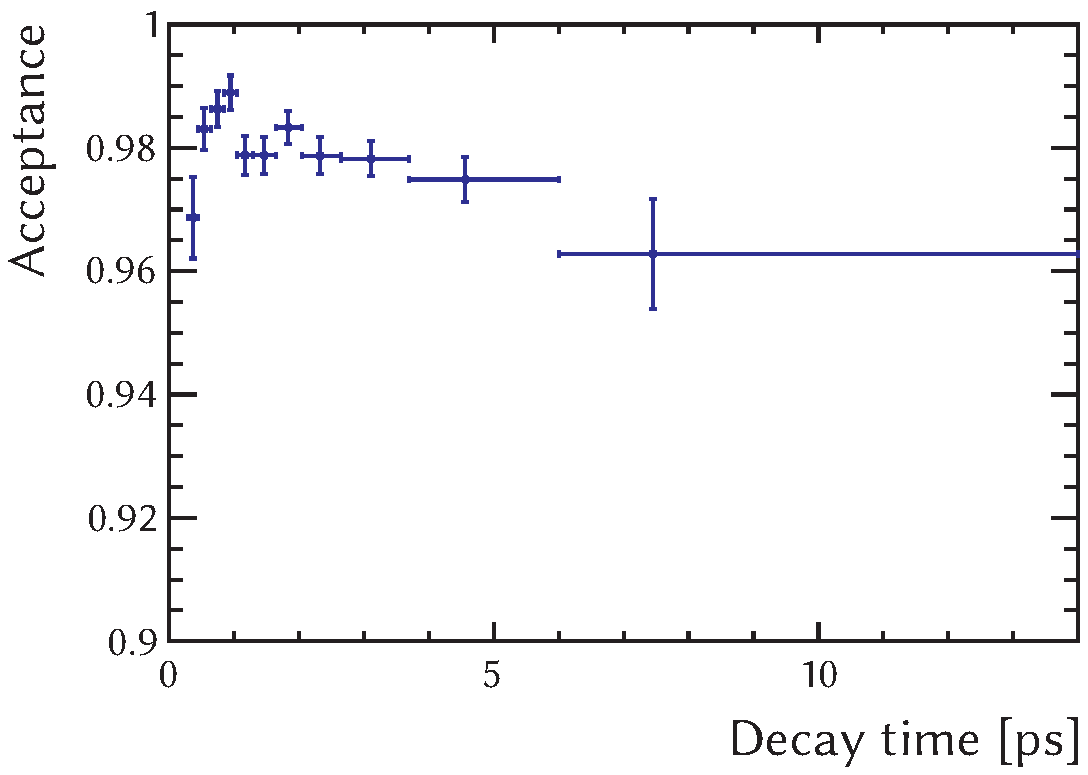
\includegraphics[width=\textwidth]{graphics/analysis/trigTimeAcc_2012_UB}
    \caption{}
    \label{fig:trigAcc_2012_UB}
  \end{subfigure}%
  \hfill%
  \begin{subfigure}{0.49\textwidth}
    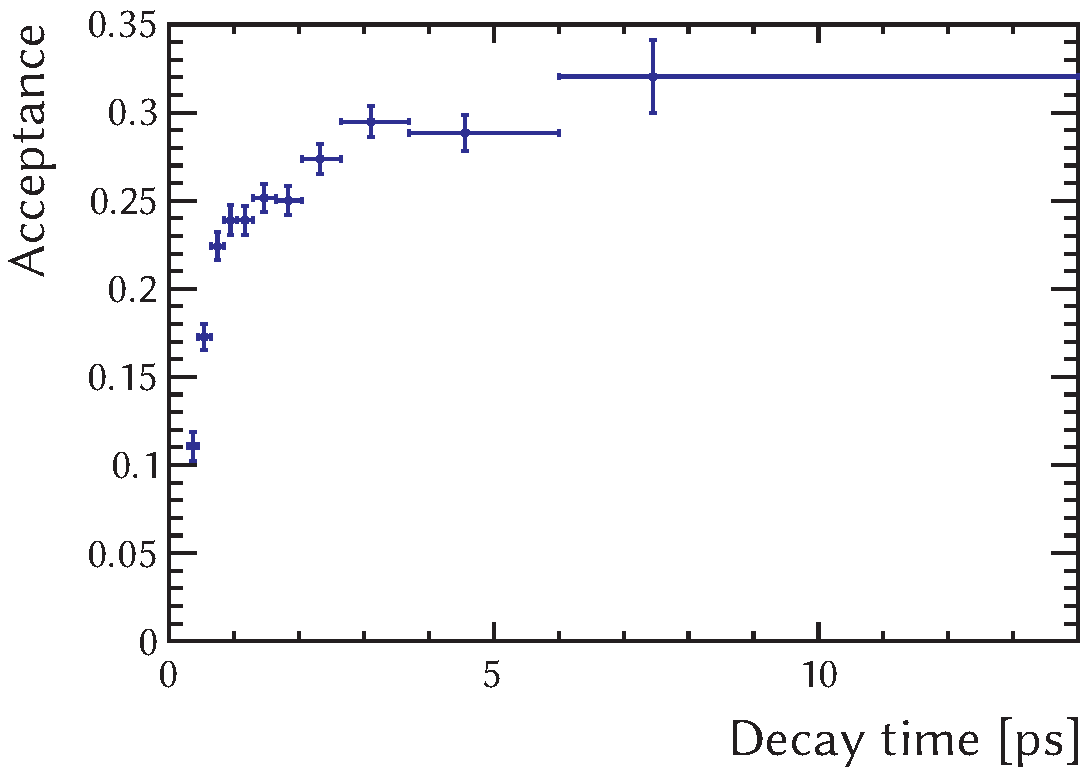
\includegraphics[width=\textwidth]{graphics/analysis/trigTimeAcc_2012_exclB}
    \caption{}
    \label{fig:trigAcc_2012_exclB}
  \end{subfigure}
  \caption{Trigger acceptance in bins of decay time for (a, b) the 2011 run and (c, d) the 2012 run
           and for (a, c) the HLT1-unbiased/HLT2-biased selection and (b, d) the exclusively-HLT1-biased/HLT2-biased selection.
           Notice that the efficiency range of the HLT1-unbiased/HLT2-biased graphs is 90--100\%.
           Because the absolute efficiency of the HLT1 selections is unknown, the scales of the efficiencies
           in the graphs are given with respect to the efficiency of the HLT1-unbiased selection.}
  \label{fig:trigAcc}
\end{figure}


\section{Decay Angles}
\label{sec:ana_angles}

Also the measurement of the decay angles has a finite precision and is affected by a non-trivial acceptance shape. Whereas resolution
effects in decay time directly affect the amplitude of the measured decay-time oscillation and, therefore, the estimates of the
CP-violation parameters, the effect of angular resolution are indirect and expected to be smaller. Because a convolution of the angular
functions in the decay model with a resolution function would be far from trivial, angular resolution is not included in the model of the
decay. However, resolution effects cannot be neglected and introduce systematic uncertainties in the final parameter estimates (see
Section~\ref{sec:result_syst}).

The acceptance as a function of decay angles is included in the decay model. Its shape is shown in Figure~\ref{fig:angAcc}. The figure
shows the acceptance function for each of three angles, integrated over the two remaining angles. The data points are sums of simulated
decays, weighted by the inverse of the PDF that was used to generate the decays at each point in decay angles. This results in the ratio of
the observed distribution including acceptance effects and the generated distribution. The shape of this ratio in the decay angles is given
by the shape of the angular acceptance function. In essence this is also how the acceptance function for the decay model, represented by
the blue line, is determined.

\begin{figure}[tbp]
  \centering
  \begin{subfigure}{0.49\textwidth}
    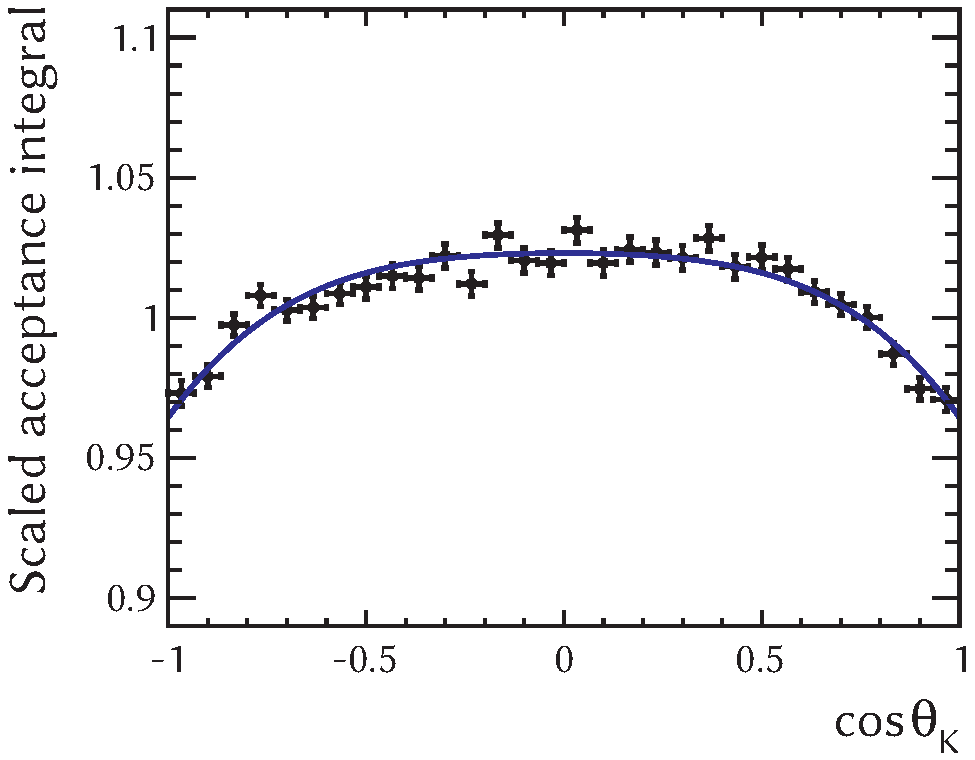
\includegraphics[width=\textwidth]{graphics/analysis/angAcc_ctk}
    \caption{}
    \label{fig:angAcc_ctk}
  \end{subfigure}%
  \hfill%
  \begin{subfigure}{0.49\textwidth}
    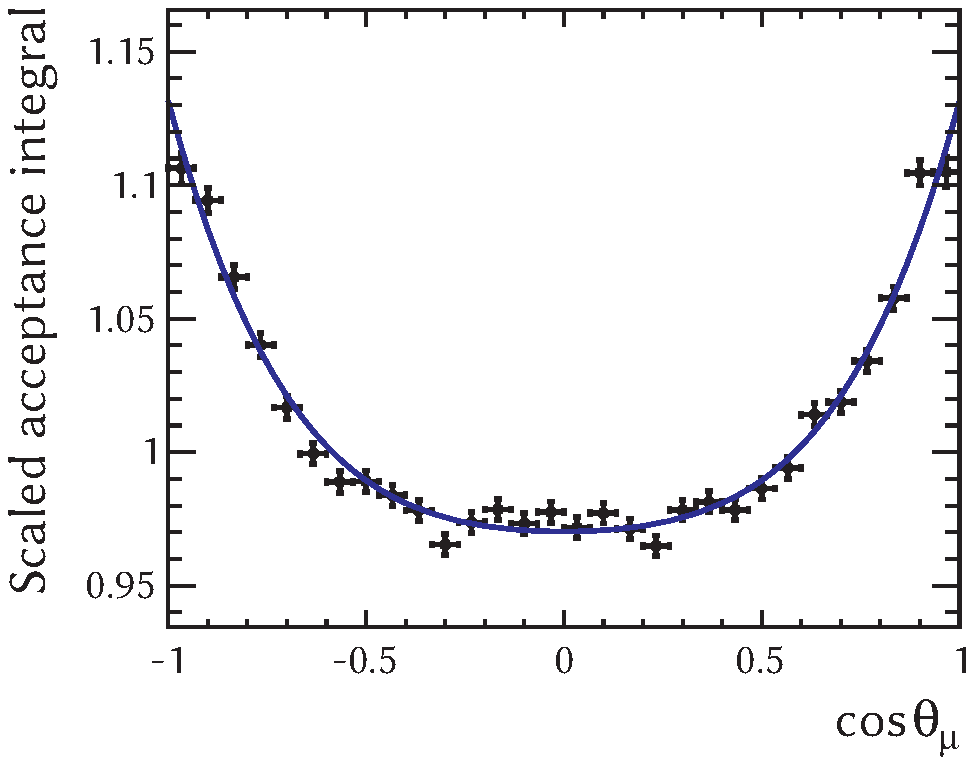
\includegraphics[width=\textwidth]{graphics/analysis/angAcc_ctl}
    \caption{}
    \label{fig:angAcc_ctl}
  \end{subfigure}

  \vspace*{0.02\textwidth}
  \begin{subfigure}{0.49\textwidth}
    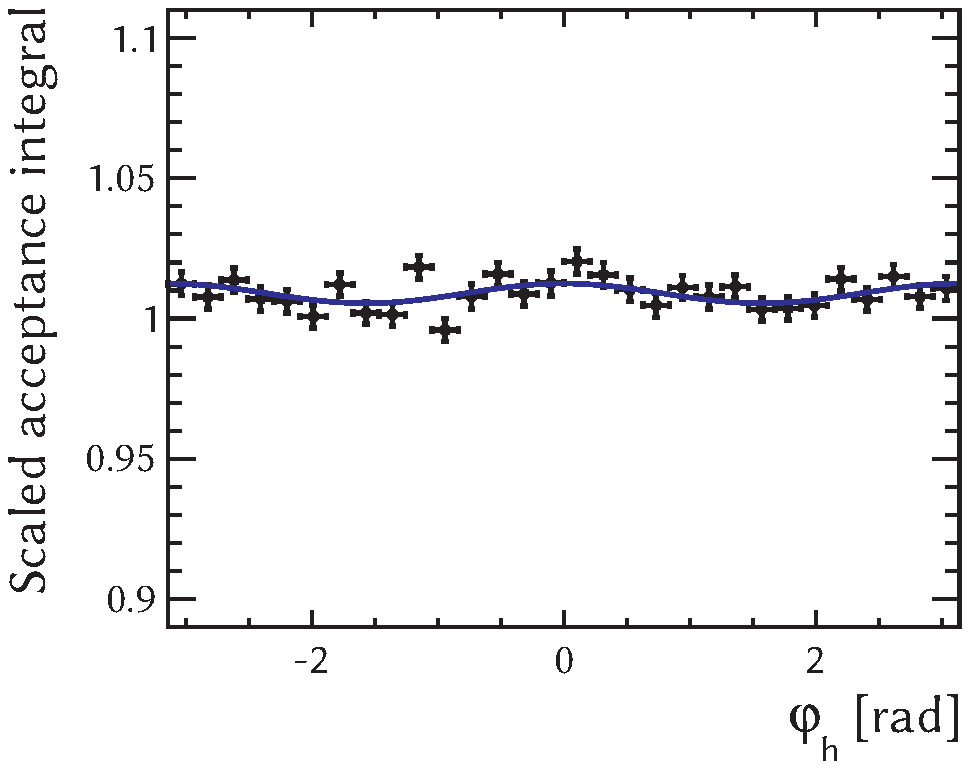
\includegraphics[width=\textwidth]{graphics/analysis/angAcc_phi}
    \caption{}
    \label{fig:angAcc_phi}
  \end{subfigure}
  \caption{Shape of the acceptance function in each of the three decay angles: (a) $\cthetaK$, (b) $\cthetal$, (c) $\phihel$.
           The angular acceptance function is integrated over the two remaining angles in each of the figures.
           The blue line represents a parameterization of the function in terms of Legendre polynomials for $\cthetaK$
           and real-valued spherical harmonics for $\cthetal$ and $\phihel$.
           The data points are obtained by a sum over simulated decays, which are weighted by the value of the PDF that was used to
           generate the decays at each point in decay angles.
           Notice that the vertical scale of these figures does not start at zero.}
  \label{fig:angAcc}
\end{figure}

The ratio of observed and generated angular PDFs can be written as
\begin{equation}
  \begin{aligned}
    \frac{P^\text{obs}(\Omega|t)}{P^\text{gen}(\Omega|t)}
        &= \frac{\effta\, p(t,\Omega)}{\int\ud\Omega\; \effta\, p(t,\Omega)}\; \frac{\int\ud\Omega\; p(t,\Omega)}{p(t,\Omega)}\\
         = &\frac{\effta\, \int\ud\Omega\; p(t,\Omega)}{\int\ud\Omega\; \effta\, p(t,\Omega)}
         = \frac{\effta}{\int\ud\Omega\; \effta\, P^\text{gen}(\Omega|t)}
         = \frac{\effta}{\meff(t)}\\
        \effta &= \meff(t)\; \frac{P^\text{obs}(\Omega|t)}{P^\text{gen}(\Omega|t)} \ ,
  \end{aligned}
  \label{eq:angAccPDFRatio}
\end{equation}
where $P^\text{obs}$ is the observed PDF, $P^\text{gen}$ the generated PDF, $p$ the function of time and angles from which the PDFs are
built, and $\eff$ the time and angular acceptance function. Both angular PDFs are conditional on decay time. The angular mean of the
acceptance function, which depends on decay time, is given by
\begin{equation}
  \meff(t) \equiv \int\ud\Omega\, \effta\, P^\text{gen}(\Omega|t)\ .
\end{equation}

Assuming the time and angular acceptance functions factorize, that is $\effta = \efft \times \effa$, the mean acceptance can be expressed
as
\begin{equation}
  \meff(t) = \efft \times \int\ud\Omega\, \effa\, P^\text{gen}(\Omega|t)
           = \efft \times \meffa(t) \ .
\end{equation}
Inserting this expression into the last line of Equation~\ref{eq:angAccPDFRatio} yields for the acceptance function
\begin{equation}
  \effta = \efft \times \meffa(t)\; \frac{P^\text{obs}(\Omega|t)}{P^\text{gen}(\Omega|t)}\ ,
\end{equation}
which means that the angular acceptance function is given by
\begin{equation}
  \label{eq:angAcc}
  \effa = \meffa(t)\; \frac{P^\text{obs}(\Omega|t)}{P^\text{gen}(\Omega|t)}\ .
\end{equation}
The factor $\meffa(t)$ is the mean of the angular acceptance function, which generally depends on decay time. Since only the shape of the
angular acceptance function is relevant in this model, it is not required to determine the value of this angular constant factor. The ratio
of the observed and generated PDFs suffices to determine the shape of the function in the decay angles.


%%%%%%%%%%%%%%%%%%%%%%%%%%%%%%%%%%%%%%%%
\subsection{Acceptance Parameterization}
\label{subsec:ana_angles_param}
%%%%%%%%%%%%%%%%%%%%%%%%%%%%%%%%%%%%%%%%

The function $\effa$ is represented in Figure~\ref{fig:angAcc} by the blue line. For this figure, it is parameterized in terms of Legendre
polynomials and real-valued spherical harmonics, $\Lp{i}(\cthetaK)\,\rsph{l}{m}(\cthetal,\phihel)$ (see also
Section~\ref{sec:angularDecay_squareAmp}, Equations~\ref{eq:PYdef} and \ref{eq:realYdef}). These functions form an orthogonal basis of
functions of the three decay angles.

In principle an arbitrary function is expressed as an infinite sum of basis functions, but in practice the relatively uniform acceptance
function can be described by a limited number of contributions. The function $\Lp{0}\,\rsph{0}{0}$ is a constant and would be the only
contribution for a truly uniform acceptance function. A few higher-order functions up to $i$\texteq4, $l$\texteq4, and $m$\texteq2 are
included to describe the shape shown in Figure~\ref{fig:angAcc}. Even higher orders represent faster changes in the acceptance function and
can be omitted for this slowly-changing shape.

The coefficients of the basis functions, which specify the shape of the acceptance function, are determined from the simulated
\BstoJpsiKK{} decays that were used for Figure~\ref{fig:angAcc}. Expressing the acceptance function as
\begin{equation}
  \effa = \sum_{i,l,m} c_{ilm}\,b_{ilm}(\Omega)\ ,
\end{equation}
the coefficients are defined as
\begin{equation}
  \label{eq:angEffCoefDef}
  c_{ilm} \equiv (i+\tfrac{1}{2}) \int\ud\Omega\,b_{ilm}(\Omega)\,\effa\ ,
\end{equation}
where $b_{ilm}$ is a basis function and $c_{ilm}$ the corresponding coefficient. The normalization factor $i+\tfrac{1}{2}$ arises from
the fact that Legendre polynomials are orthogonal, but not orthonormal:
\begin{equation}
  \int\ud\cthetaK\,\Lp{i}(\cthetaK)\cdot\Lp{i}(\cthetaK) = \frac{1}{i+\tfrac{1}{2}}\ .
\end{equation}

The integral in Equation~\ref{eq:angEffCoefDef} is calculated by means of Monte Carlo integration, using the simulated decays. A constant
is defined to absorb the factor $\meffa(t)$ in Equation~\ref{eq:angAcc}:
\begin{equation}
  \label{eq:angEffConst}
  E_a \equiv \left[ \int\ud t\, \frac{P^\text{obs}(t)}{\meffa(t)} \right]^{-1}\ .
\end{equation}
Notice that $E_a$ reduces to the mean angular acceptance, $\meffa$, if the PDFs for time and angles factorize,
$P^\text{gen}(t,\Omega)$\texteq$P^\text{gen}(t)$\texttimes$P^\text{gen}(\Omega)$. In this case $P^\text{gen}(\Omega|t)$ is equal to
$P^\text{gen}(\Omega)$ and $\meffa$ is independent of time and the integral in Equation~\ref{eq:angEffConst} evaluates to $\meffa^{-1}$.

With the constant $E_a$ and the definition of the angular acceptance in Equation~\ref{eq:angAcc}, the coefficients of
Equation~\ref{eq:angEffCoefDef} can be expressed as
\begin{equation}
  \label{eq:angAccInt}
  \begin{split}
    \tfrac{1}{E_a}\, c_{ilm} &= \int\ud t\, \frac{P^\text{obs}(t)}{\meffa(t)}
                                \cdot (i+\tfrac{1}{2}) \int\ud\Omega\,b_{ilm}(\Omega)\, \effa \\
                             &= (i+\tfrac{1}{2}) \int\ud t\, \ud\Omega\; \frac{P^\text{obs}(t)}{\meffa(t)}\,
                                b_{ilm}(\Omega)\, \meffa(t)\, \frac{P^\text{obs}(\Omega|t)}{P^\text{gen}(\Omega|t)} \\
                             &= (i+\tfrac{1}{2}) \int\ud t\, \ud\Omega\; P^\text{obs}(t,\Omega)\,
                                \frac{b_{ilm}(\Omega)}{P^\text{gen}(\Omega|t)} \ .
  \end{split}
\end{equation}
The value of this integral is estimated with a sum over simulated decays:
\begin{equation}
  E\left( \tfrac{1}{E_a}\, c_{ilm} \right)
      = (i + \tfrac{1}{2})\, \frac{1}{N^\text{obs}}\, \sum_{e=1}^{N^\text{obs}}\frac{b_{ilm}(\Omega_e)}{P^\text{gen}(\Omega_e|t_e)}
  \label{eq:angEffCoefEst}
\end{equation}
Since the ``mean acceptance'' is a constant equal for all coefficients, this factor can be ignored for the shape of the acceptance
function. The values of the coefficients that were used for the function in Figure~\ref{fig:angAcc} are specified in
Table~\ref{tab:angEffCoefs}.
\begin{table}[htbp]
  \centering
  \caption{Values of the coefficients of the angular acceptance function that were used for the function shown in Figure~\ref{fig:angAcc}.
           The specified values are estimates of the quantity $\tfrac{1}{E_a}\, c_{ilm}$ (Equation~\ref{eq:angEffCoefEst}).}
  \label{tab:angEffCoefs}
  \begin{tabular}{ccc}
    \hline
    coefficient ($ilm$)  &  value  &  statistical uncertainty  \\
    \hline
    000  &   3.5767  &  0.0011  \\
    020  &  +0.1535  &  0.0030  \\
    040  &  +0.0305  &  0.0031  \\
    022  &  +0.0096  &  0.0026  \\
    200  &  -0.125   &  0.006   \\
    400  &  -0.033   &  0.008   \\
    \hline
  \end{tabular}
\end{table}

For a uniform acceptance function, $\effa$\texteq$\meffa$\texteq constant, and Equation~\ref{eq:angAccInt} reduces to
\begin{equation}
  \tfrac{1}{E_a}\, c_{ilm} = (i+\tfrac{1}{2}) \int\ud\Omega\,b_{ilm}(\Omega)\ .
\end{equation}
This integral is only non-zero for $i$\texteq$l$\texteq$m$\texteq0, for which $\tfrac{1}{E_a}\,c_{000}$\texteq2$\sqrt{\pi}$\textapprox3.54.
Table~\ref{tab:angEffCoefs} shows that the acceptance function is not too far from being uniform.


%%%%%%%%%%%%%%%%%%%%%%%%%%%%%%%%%
\subsection{Acceptance Normalization Weights}
\label{subsec:ana_angles_weights}
%%%%%%%%%%%%%%%%%%%%%%%%%%%%%%%%%

In principle the parameterization of the acceptance function in terms of Legendre polynomials and spherical harmonics could be used to
describe the acceptance function in the PDF for the time and angular fit. However, this would require criteria that specify which set of
basis functions to include in the description and a study of the effect of not including functions that are not in this set. A slightly
different approach circumvents this problem and includes all relevant acceptance information.

Using the notation of Equation~\ref{eq:angAccPDFRatio}, the PDF including acceptance effects is given by
\begin{equation}
  \label{eq:obsPDF}
  P^\text{obs}(t,\Omega) = \frac{\effta\, p(t,\Omega)}{\int\ud t\, \ud\Omega\; \effta\, p(t,\Omega)}
\end{equation}
Assuming the time and angular acceptance functions factorize and writing the function $p(t,\Omega)$ in the normalization integral as a sum
of angular terms (see Sections~\ref{sec:pheno_angles} and \ref{sec:pheno_equations}), the PDF can be expressed as
\begin{equation}
  \label{eq:obsPDFNormSum}
  P^\text{obs}(t,\Omega) = \efft\,\effa\, \frac{p(t,\Omega)}{\sum_k \int\ud t\, \efft f_t(t) \int\ud\Omega\, \effa f_{a,k}(\Omega)}
\end{equation}

If the angular acceptance function does not contain any free parameters, the factor $\effa$ in Equation~\ref{eq:obsPDFNormSum} becomes a
constant term in the minimization of the NLL (see also Section~\ref{sec:ana_fit}) and can be ignored. The angular acceptance function then
only remains in the normalization integral $\int\ud\Omega\, \effa f_{a,k}(\Omega)$. This integral is very similar to the integral in
Equation~\ref{eq:angEffCoefDef} and can be estimated in the same way (Equations~\ref{eq:angAccInt} and \ref{eq:angEffCoefEst}).

This procedure leads to the definition of \emph{normalization weights}, which were first described in \cite{duPree:2010}. The weights are
determined for each term in the differential decay rate and are defined by
\begin{equation}
  \label{eq:angNormWeightDef}
  \xi_k \equiv \int\ud\Omega\, \effa f_{a,k}(\Omega)\ ,
\end{equation}
with a corresponding estimate from simulated events
\begin{equation}
  \label{eq:angNormWeightEst}
  E\left( \tfrac{1}{E_a}\, \xi_k \right)
      = \frac{1}{N^\text{obs}}\, \sum_{e=1}^{N^\text{obs}}\frac{f_{a,k}(\Omega_e)}{P^\text{gen}(\Omega_e|t_e)}\ .
\end{equation}
The estimated values of the normalization weights are given in Table~\ref{tab:angNormWeights}.
\begin{table}[htbp]
  \centering
  \caption{Values of the normalization weights of the angular acceptance function.
           The specified values are estimates of the quantity $\tfrac{1}{E_a}\, \xi_k$ (Equation~\ref{eq:angNormWeightEst}).}
  \label{tab:angNormWeights}
  \begin{tabular}{ccc}
    \hline
    weight ($k$)  &  value  &  statistical uncertainty  \\
    \hline
    00                    &  0.9744   &  0.0005  \\
    $\parallel\parallel$  &  1.0245   &  0.0006  \\
    $\perp\perp$          &  1.0263   &  0.0006  \\
    0$\parallel$          &  +0.0001  &  0.0005  \\
    0$\perp$              &  -0.0003  &  0.0004  \\
    $\parallel\perp$      &  -0.0006  &  0.0007  \\
    SS                    &  0.9896   &  0.0004  \\
    0S                    &  +0.0007  &  0.0014  \\
    $\parallel$S          &  +0.0007  &  0.0006  \\
    $\perp$S              &  +0.0003  &  0.0006  \\
    \hline
  \end{tabular}
\end{table}

\emph{to do:}
\begin{itemize}
  \item \emph{check signs in table}
  \item \emph{describe conversion between weights and basis coefficients}
\end{itemize}


\section{\texorpdfstring{$\KK$}{KK}-Mass Integrals}
\label{sec:ana_KKIntegrals}

\begin{itemize}
  \item PDFs conditional on $\KK$-mass bin
  \item no sensitivity to mass shape, other than bin integrals
  \item calculation of $\CSP$ factors with different models
        ($\fzero$ Flatt\'e parameters from \cite{Ablikim:2004wn}, resolution from MC)
\end{itemize}

\begin{table}[htb]
  \centering
  \caption{S-wave--$\Jpsiphi$ coupling factors in the six $\KK$-mass bins ($\CSP^i$).}
  \label{tab:CSPFactors}
  \begin{tabular}{cccc}
    bin     & nominal  &  +20\% resolution  &  uniform S-wave  \\
    \hline
    1       & 0.9178   &  0.9152            &  0.9586          \\
    2       & 0.9022   &  0.8797            &  0.9110          \\
    3       & 0.8619   &  0.8357            &  0.8618          \\
    4       & 0.8875   &  0.8599            &  0.8828          \\
    5       & 0.9360   &  0.9207            &  0.9227          \\
    6       & 0.9641   &  0.9624            &  0.9110          \\
  \end{tabular}
\end{table}

\section{Flavour Tagging}
\label{sec:ana_tagging}

In Chapter~\ref{chap:pheno} the expressions for the differential decay rates of $\Bs$ and $\Bsbar$ decays are distinguished by the
variable $\qf$, which takes the value \tp1 for $\Bs$ and \tm1 for $\Bsbar$. Equation~\ref{eq:timeqfDep} in Section~\ref{sec:pheno_time}
shows the dependence on this variable.

As explained in Section~\ref{subsec:intro_LHCb_LHC}, it is experimentally not possible to determine whether the produced meson was $\Bs$
and $\Bsbar$ for each individual decay. Instead, this meson flavour is estimated for each decay, together with a probability that the
estimate is wrong. This \emph{flavour tag} is denoted by $\qt$, which takes the values \tp1 for a $\Bs$ estimate and \tm1 for a $\Bsbar$
estimate. The estimate of the wrong-tag probability is denoted by $\etaTag$.

For either value of $\qt$ the differential rate is a sum of the rates for true $\Bs$ ($\qf$\texteq\tp1) and true $\Bsbar$
($\qf$\texteq\tm1), where the relative contributions depend on the wrong-tag probability. For small wrong-tag probability the two
contributions are well separated, which enables the measurement of the oscillation amplitude from which the main sensitivity to
CP-violation parameters originates (see Section~\ref{sec:pheno_equations}). If the wrong-tag probability becomes larger, the opposite
oscillations of true $\Bs$ and true $\Bsbar$ start to cancel.

Decay candidates are assigned to different \emph{flavour-tagging categories} according to the estimate of the wrong-tag probability. For
the main measurement the candidates are only classified as \emph{tagged} (0\textlt$\etaTag$\textle0.5) or \emph{untagged}
($\etaTag$\texteq0.5). For tagged decay candidates the decay model depends on the value of $\etaTag$ for each candidate. For untagged
candidates the flavour-tagging algorithms are unable to estimate the $\Bs$ flavour. For these candidates the wrong-tag probability is 50\%
by definition.

Although the implementation of flavour tagging that uses the value of $\etaTag$ for each individual decay candidate is more optimal, the
analysis can be simplified by using an average wrong-tag probability for tagged candidates. In this case the tagging information can be
used more optimally by defining several categories of tagged events, such that candidates with small and large wrong-tag probabilities are
separated. This is achieved by defining ranges in $\etaTag$.

In summing the contributions of true $\Bs$ and true $\Bsbar$ any asymmetries in their production and detection should be taken into
account. The LHC collides protons, which contain more matter than antimatter. This creates a small matter--antimatter asymmetry in the
fragmentation and hadronization processes and consequently a small asymmetry in the numbers of $\Bs$ and $\Bsbar$ that are produced. In
addition, the flavour-tagging process relies on the detection of charged kaons, which is asymmetric for $\Kp$ and $\Km$. This creates a
difference in the fractions of the $\Bs$ and $\Bsbar$ decays in each tagging category.


%%%%%%%%%%%%%%%%%%%%%%%%%%%%%%%
\subsection{Formalism}
\label{subsec:ana_tagging_form}
%%%%%%%%%%%%%%%%%%%%%%%%%%%%%%%

The effect of any of $\Bs$--$\Bsbar$ normalization asymmetries on the differential decay rate can be written in the form 1\textplus$\qf\,
A$, where the asymmetry is denoted by $A$. Examining Equation~\ref{eq:timeqfDep}, an additional normalization asymmetry arises from CP
violation in mixing. The factor $1-\qf\,\Cm$ is included as an asymmetry contribution, with $A$\texteq\tm$\Cm$.

Exploiting the relation $\qf^2$\texteq\tp1, the product of all asymmetries can be expressed in a general form as
\begin{equation}
  \label{eq:asymProd}
  \prod_i (1+\qf\, A_i) \equiv \avgCEven + \qf\,\avgCOdd \ ,
\end{equation}
where $\avgCEven$ and $\avgCOdd$ are factors that contain the asymmetries, but not the variable $\qf$. Denoting the $\cDGs$ and $\sDGs$
terms as $\even$ (even under $\Bs\leftrightarrow\Bsbar$) and the $\cDms$ and $\sDms$ terms as $\odd$ (odd under
$\Bs\leftrightarrow\Bsbar$), the differential decay rate can be expressed as
\begin{equation}
  \label{eq:diffRateAsym}
  \begin{aligned}
    \frac{\ud^4\Gamma}{\ud t\, \ud\Omega}
      &= (\avgCEven + \qf\,\avgCOdd) (\even + \qf\,\odd) \\
      &= (\avgCEven + \qf\,\avgCOdd)\, \even + (\avgCOdd + \qf\,\avgCEven)\, \odd \ .
  \end{aligned}
\end{equation}

The two tagging algorithms that are used for the \BstoJpsiKK{} measurement give separate estimates of the $\Bs$ flavour and the
corresponding wrong-tag probability. The true wrong-tag probability for $\Bs$, which is a function of the estimated probability $\etaTag$,
is denoted by $\wTag$. Because of the $\Bs$--$\Bsbar$ asymmetries mentioned above, the probability for $\Bsbar$ decays has a different
dependence on $\etaTag$ and is denoted by $\wTagBar$.

Expressions for the differential rates of different combinations of opposite-side and same-side flavour tags can be derived by multiplying
the rates for true $\Bs$ and true $\Bsbar$ by the appropriate combinations of wrong-tag probabilities. Assuming the probabilities for the
opposite-side and same-side algorithms are uncorrelated and labelling the algorithms by ``o'' and ``s'', respectively, the resulting
rates are given by
\begin{alignat}{3}
  \label{eq:diffRateWTag}
  \qtOS=+1;\, \qtSS=-1:  &\quad&  (1-\wTagOS)(1-\wTagSS)           &\;& (\avgCEven+\avgCOdd)(\even+\odd) & \nonumber\\*
                         &     &  +\ \wTagBarOS\, \wTagBarSS       &  & (\avgCEven-\avgCOdd)(\even-\odd) & \nonumber\\
  \qtOS=+1;\, \qtSS=-1:  &     &  (1-\wTagOS)\, \wTagSS            &  & (\avgCEven+\avgCOdd)(\even+\odd) & \nonumber\\*
                         &     &  +\ \wTagBarOS\, (1-\wTagBarSS)   &  & (\avgCEven-\avgCOdd)(\even-\odd) & \nonumber\\
  \qtOS=-1;\, \qtSS=+1:  &     &  \wTagSS\, (1-\wTagOS)            &  & (\avgCEven+\avgCOdd)(\even+\odd) &          \\*
                         &     &  +\ (1-\wTagBarSS)\, \wTagBarOS   &  & (\avgCEven-\avgCOdd)(\even-\odd) & \nonumber\\
  \qtOS=-1;\, \qtSS=-1:  &     &  \wTagSS\, \wTagOS                &  & (\avgCEven+\avgCOdd)(\even+\odd) & \nonumber\\*
                         &     &  +\ (1-\wTagBarSS)(1-\wTagBarOS)  &  & (\avgCEven-\avgCOdd)(\even-\odd) & \nonumber\ .
\end{alignat}
Notice that the sum of the rates of the four cases is given by the expression in Equation~\ref{eq:diffRateAsym}, summing the rates of
$\qf$\texteq\tp1 and $\qf$\texteq\tm1.

Rewriting the expressions in Equation~\ref{eq:diffRateWTag}, the observed differential decay rate in one of the tagging categories can be
expressed in a form similar to Equation~\ref{eq:diffRateAsym}:
\begin{equation}
  \label{eq:diffRateTags}
  \left(\frac{\ud^4\Gamma}{\ud t\, \ud\Omega}\right)_{c,\,\qtOS,\,\qtSS}
      = \tagCatCoef[c]\, (\CEven\, \even + \COdd\, \odd) \ ,
\end{equation}
where the coefficients $\CEven$ and $\COdd$ both depend on the tagging category, $c$, and on the flavour tags, $\qtOS$ and $\qtSS$. The
parameter $\tagCatCoef[c]$ is the average of the fractions of true $\Bs$ and true $\Bsbar$ decays in the category. To express the
coefficients in terms of these quantities, a \emph{tagging-dilution factor} and a corresponding ``asymmetry'' are defined as
\begin{equation}
  \dil = 1 - \wTag - \wTagBar  \qquad\text{and}\qquad  \ADilWTag = \frac{\wTag-\wTagBar}{1 - \wTag - \wTagBar} \ .
\end{equation}
In general, all tagging parameters depend on the tagging category: $\dil[c]$, $\ADilWTag[c]$, $\avgCEven[c]$, and $\avgCOdd[c]$. In terms
of these parameters the coefficients $\CEven$ and $\COdd$ are given by
\begin{subequations}
  \label{eq:evenOddTagCoefs}
  \begin{align}
    2\,\CEven &\equiv \avgCEven[c]
                         + \qtOS\,\dilOS[c]\left(\avgCOdd[c] - \ADilWTagOS[c]\,\avgCEven[c] \right)
                         + \qtSS\,\dilSS[c]\left(\avgCOdd[c] - \ADilWTagSS[c]\,\avgCEven[c] \right) \nonumber\\
                         &\qquad\quad\
                           + \qtOS\,\qtSS\,\dilOS[c]\,\dilSS[c]\left[(1 + \ADilWTagOS[c]\,\ADilWTagSS[c])\,\avgCEven[c]
                                                                  - \ADilWTagOS[c]\,\ADilWTagSS[c]\,\avgCOdd[c] \right] \\
    2\,\COdd &\equiv \avgCOdd[c]
                        + \qtOS\,\dilOS[c]\left(\avgCEven[c] - \ADilWTagOS[c]\,\avgCOdd[c] \right)
                        + \qtSS\,\dilSS[c]\left(\avgCEven[c] - \ADilWTagSS[c]\,\avgCOdd[c] \right) \nonumber\\
                        &\qquad\quad\
                          + \qtOS\,\qtSS\,\dilOS[c]\,\dilSS[c]\left[(1 + \ADilWTagOS[c]\,\ADilWTagSS[c])\,\avgCOdd[c]
                                                                  - \ADilWTagOS[c]\,\ADilWTagSS[c]\,\avgCEven[c] \right] \ .
  \end{align}
\end{subequations}

Various limits can be considered for the $\CEven$ and $\COdd$ coefficients in Equations~\ref{eq:diffRateTags} and \ref{eq:evenOddTagCoefs}.
Without \BsBsbar{} normalization asymmetries the coefficients $\avgCEven$ and $\avgCOdd$ reduce to one and zero, respectively:
\begin{subequations}
  \begin{align}
    2\,\CEven &= 1
                 - \qtOS\,\dilOS[c]\,\ADilWTagOS[c]
                 - \qtSS\,\dilSS[c]\,\ADilWTagSS[c]
                 + \qtOS\,\qtSS\,\dilOS[c]\,\dilSS[c]\,(1 + \ADilWTagOS[c]\,\ADilWTagSS[c]) \\
    2\,\COdd &=  \qtOS\,\dilOS[c]
                 + \qtSS\,\dilSS[c]
                 - \qtOS\,\qtSS\,\dilOS[c]\,\dilSS[c]\,\ADilWTagOS[c]\,\ADilWTagSS[c] \ .
  \end{align}
\end{subequations}
Without any asymmetries, the coefficients are given by
\begin{subequations}
  \label{eq:evenOddTagCoefsNoAsym}
  \begin{align}
    2\,\CEven &= 1
                 + \qtOS\,\qtSS\,\dilOS[c]\,\dilSS[c] \\
    2\,\COdd &=  \qtOS\,\dilOS[c]
                 + \qtSS\,\dilSS[c] \ .
  \end{align}
\end{subequations}

In case only one of the two flavour tags is considered, the differential rate is given by the sum of the $\Bs$ and $\Bsbar$ rates of the
other tag. Considering only opposite-side tagging gives
\begin{subequations}
  \begin{align}
    \sum_{\qtSS} \CEven &= \avgCEven[c] + \qtOS\,\dilOS[c]\left(\avgCOdd[c]  - \ADilWTagOS[c]\,\avgCEven[c] \right) \\
    \sum_{\qtSS} \COdd  &= \avgCOdd[c]  + \qtOS\,\dilOS[c]\left(\avgCEven[c] - \ADilWTagOS[c]\,\avgCOdd[c]  \right) \ .
  \end{align}
\end{subequations}
Effectively this is the same as considering the candidates untagged for the same-side algorithm, which gives
$\wTag$\textequiv$\wTagBar$\textequiv0.5\textto$\dil$\texteq0. Without any flavour tags the coefficients are given by
\begin{subequations}
  \begin{align}
    \sum_{\qtOS,\qtSS} \CEven &= 2\,\avgCEven[c] \\
    \sum_{\qtOS,\qtSS} \COdd  &= 2\,\avgCOdd[c]  \ .
  \end{align}
\end{subequations}

Note that without flavour tagging, one is generally not interested in an expression of the differential decay rate that depends on the
tagging category. The sum of all rates cannot depend on flavour-tagging variables or parameters and should be given by
\begin{equation}
  \sum_{c,\,\qtOS,\,\qtSS} \left(\frac{\ud^4\Gamma}{\ud t\, \ud\Omega}\right)_{c,\qtOS,\qtSS}
    = 2\,\avgCEven[\text{S}]\, \even + 2\,\avgCOdd[\text{S}]\, \odd \ ,
\end{equation}
where the coefficients $\avgCEven[\text{S}]$ and $\avgCOdd[\text{S}]$ are defined as in Equation~\ref{eq:asymProd}, but including only
asymmetries that do not depend on tagging. As a result, the weighted sums of asymmetry coefficients over tagging categories are given by
\begin{equation}
  \label{eq:avgCEvenOddSums}
  \sum_c \tagCatCoef[c]\, \avgCEven[c] = \avgCEven[\text{S}]
  \qquad\text{and}\qquad
  \sum_c \tagCatCoef[c]\, \avgCOdd[c] = \avgCOdd[\text{S}] \ .
\end{equation}

The above relations follow from the requirement that the fractions of true $\Bs$ and true $\Bsbar$ decays in the tagging categories both
add up to one:
\begin{equation}
  \sum_c \tagCatCoef[c]\,\prod_l (1+\qf\, A_{c,l}) \equiv 1
\end{equation}
for both values of $\qf$, where $l$ only iterates over category-dependent asymmetries, $A_{c,l}$. With this requirement the sum of
coefficients is given by
\begin{equation}
  \label{eq:tagCatFracsSum}
  \begin{aligned}
    \sum_c \tagCatCoef[c]\, (\avgCEven[c]+\qf\,\avgCOdd[c])
      &= \sum_c \tagCatCoef[c] \prod_k (1+\qf\,A_k) \prod_l (1+\qf\,A_{c,l}) \\
      &= \prod_k (1+\qf\,A_k)\, \sum_c \tagCatCoef[c] \prod_l (1+\qf\,A_{c,l}) \\
      &= (\avgCEven[\text{S}] + \qf\,\avgCOdd[\text{S}])\, \sum_c \tagCatCoef[c] \prod_l (1+\qf\,A_{c,l}) \\
      &= \avgCEven[\text{S}] + \qf\,\avgCOdd[\text{S}] \ ,
  \end{aligned}
\end{equation}
where $k$ iterates over asymmetries that do not depend on the tagging category, $A_k$. The relations in Equation~\ref{eq:avgCEvenOddSums}
follow from Equation~\ref{eq:tagCatFracsSum}.


%%%%%%%%%%%%%%%%%%%%%%%%%%%%%%%
\subsection{Implementation}
\label{subsec:ana_tagging_impl}
%%%%%%%%%%%%%%%%%%%%%%%%%%%%%%%

For the main measurement the data and the decay model are split into the four tagging categories that are listed in
Table~\ref{tab:tagCats}. The categories are combinations of the tagged and untagged categories for the opposite-side and same-side
algorithms. The second column in the table gives the number of signal decays in each of the categories and the third column the effective
fraction of perfectly tagged decays.
\begin{table}[htb]
  \centering
  \caption{Definition of the flavour-tagging categories.}
  \label{tab:tagCats}
  \begin{tabular}{ccc}
    \hline
    category                  &  decays [\tenpow{3}]  &  effective fraction  \\
    \hline
    untagged                  &  31                   &  0                   \\
    OS tagged -- SS untagged  &  13                   &  1.2\%               \\
    OS untagged -- SS tagged  &  34                   &  0.8\%               \\
    OS tagged -- SS tagged    &  16                   &  1.7\%               \\
    \hline
  \end{tabular}
\end{table}

The fraction of perfectly tagged decays is obtained by multiplying the fraction of decays in a category by the mean of the squared dilution
factor, $\langle{\dil[c][]}^2\rangle$. Ignoring normalization and wrong-tag asymmetries, the oscillatory terms in the differential decay
rate, from which the main sensitivity to CP-violation parameters originates, are proportional to the dilution factor
(Equations~\ref{eq:diffRateTags} and \ref{eq:evenOddTagCoefsNoAsym}). With a non-zero wrong-tag probability the value of this factor is
between plus and minus one, which makes the measured oscillation amplitudes for $\Bs$ and $\Bsbar$ tags smaller than the underlying
amplitudes for true $\Bs$ and $\Bsbar$ decays.

As a result, the uncertainties on the derived underlying amplitudes are a factor $\frac{1}{\dil[c]}$ larger than the uncertainties on the
measured amplitudes, for a single value of the wrong-tag probability. Accounting for decays with different wrong-tag probabilities and
assuming the statistical uncertainty of the measured oscillation amplitude is inversely proportional to square root of the number of decays
in the category, the decrease in precision due to wrong tags can be effectively described by a decrease in number of perfectly tagged
decays by a factor $\langle{\dil[c][]}^2\rangle$.

The $\etaTag$ dependence of the wrong-tag probabilities for tagged decays, which enters the differential rates through the factors $\dil$
and $\ADilWTag$, is described by a phenomenological model:
\begin{subequations}
  \begin{align}
    \wTag &= \pTag[0]    + \pTag[1]\,    (\etaTag-\langle\etaTag\rangle) \\
    \wTag &= \pTagBar[0] + \pTagBar[1]\, (\etaTag-\langle\etaTag\rangle) \,
  \end{align}
\end{subequations}
where $\langle\etaTag\rangle$ is the mean value of $\etaTag$ for tagged decays. The parameters $\pTag[0]$, $\pTagBar[0]$, $\pTag[1]$,
$\pTagBar[1]$ are are measured in the flavour-tagging calibration procedure and have different values for the opposite-side and same-side
algorithms. The wrong-tag probabilities for untagged decays are given by $\wTag$\textequiv$\wTagBar$\textequiv0.5.

\textit{discuss floating tagging-calibration parameters and their values}

\textit{discuss $\etaOS$ and $\etaSS$ distributions (adjust plot labels)}
\begin{figure}[htbp]
  \centering
  \begin{subfigure}{0.49\textwidth}
    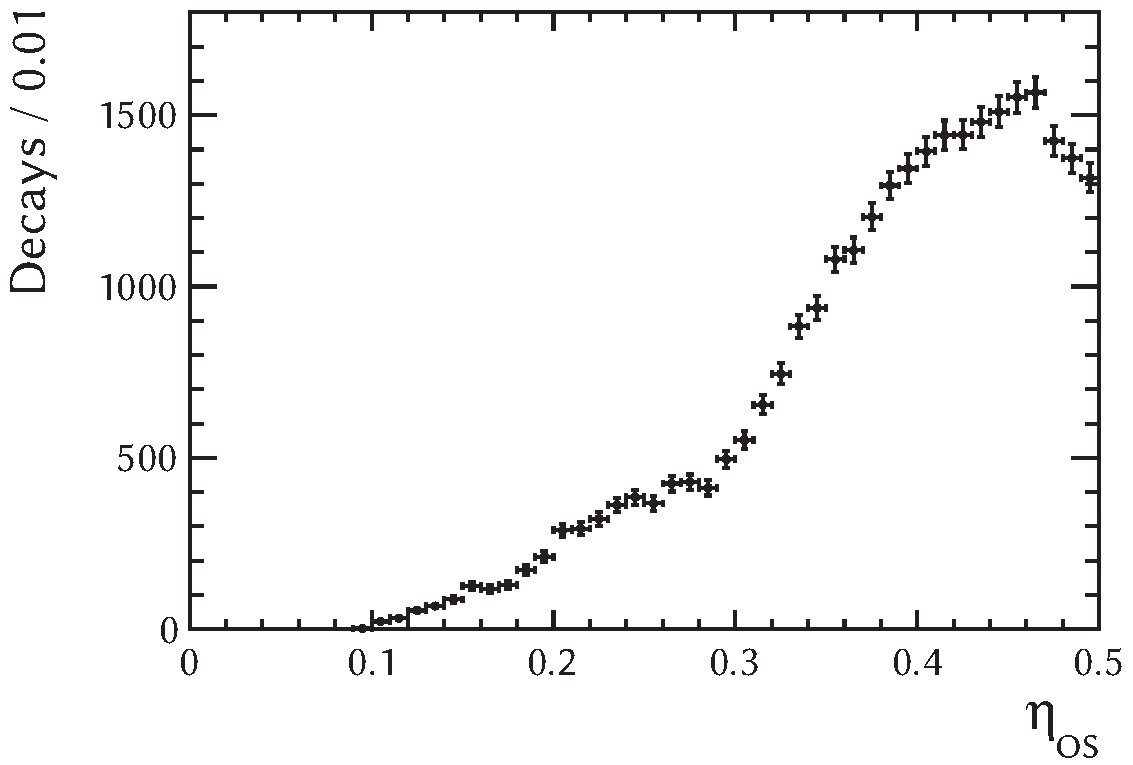
\includegraphics[width=\textwidth]{graphics/analysis/etaOS}
    \caption{}
    \label{fig:etaOS}
  \end{subfigure}%
  \hfill%
  \begin{subfigure}{0.49\textwidth}
    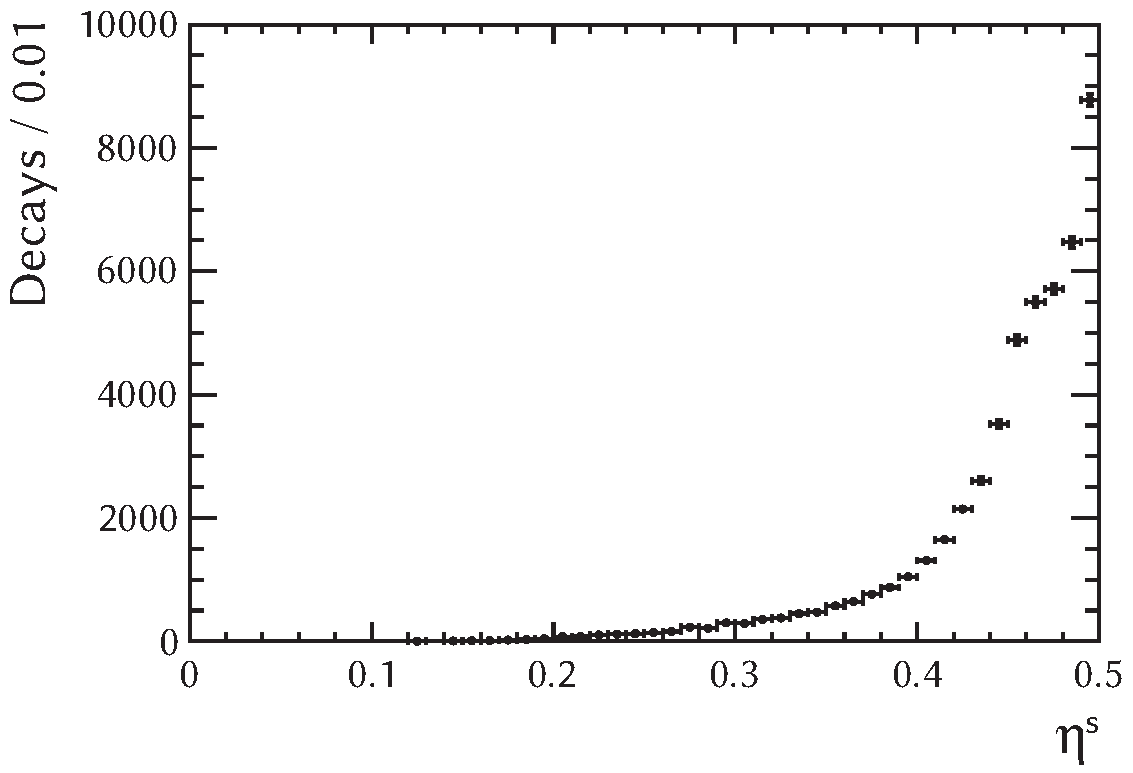
\includegraphics[width=\textwidth]{graphics/analysis/etaSS}
    \caption{}
    \label{fig:etaSS}
  \end{subfigure}
  \caption{Distribution of \BstoJpsiKK{} signal decays in the estimated wrong-tag probability
           for (a) opposite-side tagging and (b) same-side tagging.
           The contributions of untagged decays ($\etaTag$\textequiv0.5) are not shown.}
  \label{fig:etaDists}
\end{figure}

An individually normalized PDF is used for each tagging category to be insensitive to the fractions of decays in the categories, for which
there are no predictions. Since also the distributions in estimated wrong-tag probability are unpredicted, the PDFs are also made
conditional on this variable and normalized individually with respect to decay time and decay angles for each combination of $\etaOS$ and
$\etaSS$ values.

To reduce the sensitivity to \BsBsbar{} normalization asymmetries, the PDFs are also made conditional on the estimates of the $\Bs$
flavour, $\qtOS$ and $\qtSS$.
\textit{discuss why this reduces sensitivity on asymmetries}


\section{Simulation}
\label{sec:ana_sim}
\begin{itemize}
  \item \underline{briefly} discuss detector simulation
  \item toys: generate signal with model and background with real side-band data
  \item candidate weights and conditional observables in toys from fit dataset
\end{itemize}
